\RequirePackage[l2tabu,orthodox]{nag}
% chktex-file 17

\documentclass[headsepline,footsepline,footinclude=false,fontsize=11pt,paper=a4,oneside,listof=totoc,bibliography=totoc]{scrbook}

\PassOptionsToPackage{table,svgnames,dvipsnames}{xcolor}

\usepackage[utf8]{inputenc}
\usepackage[T1]{fontenc}
\usepackage[sc]{mathpazo}
\usepackage[ngerman,american]{babel}
\usepackage[autostyle]{csquotes}
\usepackage[%
  backend=biber,
  url=false,
  style=alphabetic,
  maxnames=4,
  minnames=3,
  maxbibnames=99,
  giveninits,
  uniquename=init]{biblatex}
\usepackage{url}
\setcounter{biburllcpenalty}{7000}
\setcounter{biburlucpenalty}{8000} % break urls in bibliography
\usepackage{graphicx}
\usepackage{scrhack} % necessary for listings package
\usepackage{listings}
\usepackage{lstautogobble}
\usepackage{tikz}
\usetikzlibrary{fit, positioning, shapes}
\usepackage{pgfplots}
\usepackage{pgfplotstable}
\usepackage{booktabs}
\usepackage{float} % require by the H-argument of figure e.g. \begin{figure}[H]
\usepackage[final]{microtype}
\usepackage[hidelinks]{hyperref} % hidelinks removes colored boxes around references and links
\usepackage[printonlyused]{acronym}
\usepackage{enumitem}
\usepackage{caption}
\usepackage{subcaption}
\usepackage{perpage}
\MakePerPage{footnote} % reset footnotes each page



\bibliography{bibliography}

\setkomafont{disposition}{\normalfont\bfseries} % use serif font for headings
\linespread{1.05} % adjust line spread for mathpazo font
\setlength\parindent{0pt} % remove indents
\setlength\parskip{1ex} %TODO: is this legal?

% Add table of contents to PDF bookmarks
\BeforeTOCHead[toc]{{\cleardoublepage\pdfbookmark[0]{\contentsname}{toc}}}

% Define TUM corporate design colors
% Taken from http://portal.mytum.de/corporatedesign/index_print/vorlagen/index_farben
\definecolor{TUMBlue}{HTML}{0065BD}
\definecolor{TUMSecondaryBlue}{HTML}{005293}
\definecolor{TUMSecondaryBlue2}{HTML}{003359}
\definecolor{TUMBlack}{HTML}{000000}
\definecolor{TUMWhite}{HTML}{FFFFFF}
\definecolor{TUMDarkGray}{HTML}{333333}
\definecolor{TUMGray}{HTML}{808080}
\definecolor{TUMLightGray}{HTML}{CCCCC6}
\definecolor{TUMAccentGray}{HTML}{DAD7CB}
\definecolor{TUMAccentOrange}{HTML}{E37222}
\definecolor{TUMAccentGreen}{HTML}{A2AD00}
\definecolor{TUMAccentLightBlue}{HTML}{98C6EA}
\definecolor{TUMAccentBlue}{HTML}{64A0C8}

% Settings for pgfplots
\pgfplotsset{compat=newest}
\pgfplotsset{
  % For available color names, see http://www.latextemplates.com/svgnames-colors
  cycle list={TUMBlue\\TUMAccentOrange\\TUMAccentGreen\\TUMSecondaryBlue2\\TUMDarkGray\\},
}

% Settings for lstlistings
\lstset{%
  basicstyle=\ttfamily,
  columns=fullflexible,
  autogobble,
  keywordstyle=\bfseries\color{TUMBlue},
  stringstyle=\color{TUMAccentGreen}
}

% Defined JavaScript lstlisting language
\definecolor{lightgray}{rgb}{.97,.97,.97}
\definecolor{darkgray}{rgb}{.4,.4,.4}
\definecolor{purple}{rgb}{0.65, 0.12, 0.82}

% chktex-file 18
\lstdefinelanguage{JavaScript}{
  keywords={break, case, catch, continue, debugger, default, delete, do, else, false, finally, for, function, if, in, instanceof, new, null, return, switch, this, throw, true, try, typeof, var, let, const, void, while, with},
  morecomment=[l]{//},
  morecomment=[s]{/*}{*/},
  morestring=[b]',
  morestring=[b]",
  morestring=[b]'',
  ndkeywords={class, export, boolean, throw, implements, import, this},
  keywordstyle=\color{blue}\bfseries,
  ndkeywordstyle=\color{darkgray}\bfseries,
  identifierstyle=\color{black},
  commentstyle=\color{purple}\ttfamily,
  stringstyle=\color{red}\ttfamily,
  sensitive=true
}

\lstset{
  backgroundcolor=\color{lightgray},
  extendedchars=true,
  basicstyle=\footnotesize\ttfamily,
  showstringspaces=false,
  showspaces=false,
  numbers=left,
  numberstyle=\footnotesize,
  numbersep=9pt,
  tabsize=2,
  breaklines=true,
  showtabs=false,
  captionpos=b
}


\newcommand*{\getUniversity}{Technical University of Munich}
\newcommand*{\getFaculty}{Informatics}
\newcommand*{\getStudies}{Informatics: Games Engineering}
\newcommand*{\getTitle}{Smartphone-Assisted Virtual Reality\newline Using Ubi-Interact}
\newcommand*{\getTitleGer}{Smartphone-gestützte Virtuelle Realität\newline mit Ubi-Interact}
\newcommand*{\getAuthor}{Michael Lohr}
\newcommand*{\getDoctype}{Bachelor's Thesis}
\newcommand*{\getSupervisor}{Prof.\ Gudrun Johanna Klinker, Ph.D.}
\newcommand*{\getAdvisor}{Sandro Weber, M.Sc.}
\newcommand*{\getSubmissionDate}{October 15, 2019}
\newcommand*{\getSubmissionLocation}{Munich}

\begin{document}

% Set page numbering to avoid "destination with the same identifier has been already used" warning for cover page.
% (see https://en.wikibooks.org/wiki/LaTeX/Hyperlinks#Problems_with_Links_and_Pages).
\pagenumbering{alph}
% !TeX root = ../main.tex
\begin{titlepage}
  % HACK for two-sided documents: ignore binding correction for cover page.
  % Adapted from Markus Kohm's KOMA-Script titlepage=firstiscover handling.
  % See http://mirrors.ctan.org/macros/latex/contrib/koma-script/scrkernel-title.dtx,
  % \maketitle macro.
  \oddsidemargin=\evensidemargin\relax
  \textwidth=\dimexpr\paperwidth-2\evensidemargin-2in\relax
  \hsize=\textwidth\relax

  \centering

  
\includegraphics[height=20mm]{logos/tum.pdf}

  \vspace{5mm}
  {\huge\MakeUppercase{Department of \getFaculty{}}}\\

  \vspace{5mm}
  {\large\MakeUppercase{\getUniversity{}}}\\

  \vspace{20mm}
  {\Large \getDoctype{} in \getStudies{}}

  \vspace{15mm}
  {\huge\bfseries \getTitle{}}

  \vspace{15mm}
  {\LARGE \getAuthor{}}

  \IfFileExists{logos/faculty.png}{%
    \vfill{}
    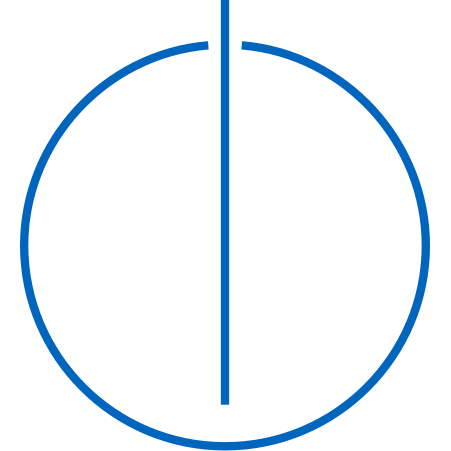
\includegraphics[height=20mm]{logos/faculty.png}
  }{}
\end{titlepage}


\frontmatter{}

% order: % https://gradschool.unc.edu/academics/thesis-diss/guide/ordercomponents.html
\begin{titlepage}
  \centering

  
\includegraphics[height=20mm]{logos/tum.pdf}

  \vspace{5mm}
  {\huge\MakeUppercase{Department of \getFaculty{}}}\\

  \vspace{5mm}
  {\large\MakeUppercase{\getUniversity{}}}\\

  \vspace{20mm}
  {\Large \getDoctype{} in \getStudies{}}

  \vspace{15mm}
  {\huge\bfseries \getTitle{}}

  \vspace{10mm}
  {\huge\bfseries \foreignlanguage{ngerman}{\getTitleGer{}}}

  \vspace{15mm}
  \begin{tabular}{l l}
    Author:          & \getAuthor{} \\
    Supervisor:      & \getSupervisor{} \\
    Advisor:         & \getAdvisor{} \\
    Submission Date: & \getSubmissionDate{} \\
  \end{tabular}

  \IfFileExists{logos/faculty.png}{%
    \vfill{}
    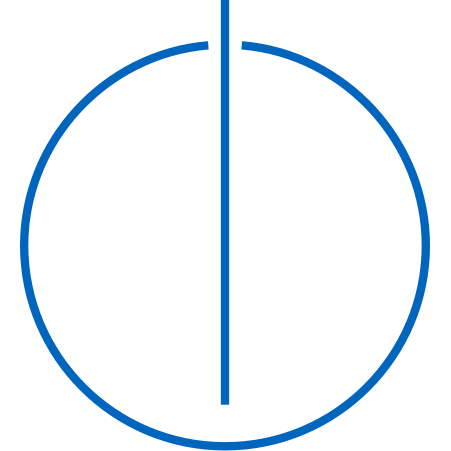
\includegraphics[height=20mm]{logos/faculty.png}
  }{}
\end{titlepage}

% !TeX root = ../main.tex
\thispagestyle{empty}
\vspace*{0.75\textheight}
\noindent
I confirm that this \MakeLowercase{\getDoctype{}} is my own work and I have documented all sources and material used.

\vspace*{1.5cm}  % leave some space above the horizontal line
\hrule
\noindent
\begin{minipage}[t]{0.4\textwidth}
    \vspace{2mm} % just a bit more whitespace below the line
    \getSubmissionLocation{}, \getSubmissionDate{} 
\end{minipage}
\hspace{1.5cm}
\begin{minipage}[t]{0.4\textwidth}
    \vspace{2mm} % just a bit more whitespace below the line
    \getAuthor{}
\end{minipage}

\hspace{50mm}

\cleardoublepage{}

\chapter{\abstractname}

%TODO: Abstract


% English



% German



\microtypesetup{protrusion=false} % disable for lists: http://www.khirevich.com/latex/microtype/
\tableofcontents{}
\microtypesetup{protrusion=true}
% !TeX root = ../main.tex
\chapter{Abbreviations}

% https://tex.stackexchange.com/questions/70875/how-to-render-individual-acronyms-in-lower-case-when-used-inline-but-mixed-case
\makeatletter
\newif\if@in@acrolist % chktex 1
\AtBeginEnvironment{acronym}{\@in@acrolisttrue}
\newrobustcmd{\LU}[2]{\if@in@acrolist#1\else#2\fi}
\begin{acronym}

	% use to sort: https://codebeautify.org/sort-text-lines
	% check for correct alphabetical order
	\acro{API}{Application Programming Interface}
	\acro{AR}{Augmented Reality}
	\acrodefplural{DOF}[DOF]{Degrees Of Freedom}
	\acro{DOF}{Degree Of Freedom}
	\acro{HMD}{Head-Mounted Display}
	\acro{IMU}{Inertial Measurement Unit}
	\acro{JS}{JavaScript}
	\acro{LAN}{Local Area Network}
	\acro{MR}{Mixed Reality}
	\acro{OS}{Operating System}
	\acro{PC}{Personal Computer}
	\acro{Protobuf}{Google Protocol Buffers}
	\acro{STD}[SD]{Standard Deviation}
	\acro{SUS}{System Usability Scale}
	\acro{UBII}{Ubi-Interact}
	\acro{UID}{Unique Identifier}
	\acro{UI}{User Interface}
	\acro{VE}{Virtual Environment}
	\acro{VR}{Virtual Reality}
	\acro{WLAN}{Wireless Local Area Network}

	\acro{2D}{\LU{T}{t}wo-dimensional}
	\acro{3D}{\LU{T}{t}hree-dimensional}

\end{acronym}


\mainmatter{}

% !TeX root = ../main.tex
\chapter{Introduction}\label{chapter:introduction}

\section{Motivation}\label{section:motivation}

\ac{VR} is an emerging technology, which provides new ways to present and interact with digital information. \citeauthor{Sherman.2003} define \ac{VR} by the four key elements virtual world, immersion, sensory feedback, and interactivity. The virtual world is an imaginary space which may be manifested through a medium. It is also described as a description of objects in a space together with rules and relationships. According to the author,  immersion means the feeling of presence in a virtual world. An essential ingredient to \ac{VR} is the sensory feedback, which describes the feedback the \ac{VR} system conveys to the user depending on the user's state in the virtual world. \ac{VR} should respond to the user's actions to make it interactive, in order for \ac{VR} to seem authentic.
These four elements form the definition as a medium composed of interactive computer simulations that may sense the user's behavior and replace or augment the sensory feedback, with the goal of immersing the user in a virtual world~\cite[6-12]{Sherman.2003}.

A \ac{HMD} as the display device, connected to a \ac{PC} which processes the data, is required for modern consumer \ac{VR} systems. Often an external tracking system is required, too.

Experiencing \acp{VE} using a \ac{VR} headset (or \ac{HMD}) is a great experience. But \ac{VR} really shines when interactivity comes into play. Since consumer \acp{HMD} are now available, the development of tracked hand controllers (also known as \ac{VR}/\ac{3D}/hand/motion controllers) gets more important.
Best practices are not yet defined, which leaves much room for new methods and research. Figure~\ref{fig:vr-controllers} illustrates the variety of different consumer \ac{VR} controllers available.

\begin{figure}[H]%
	\centering%
	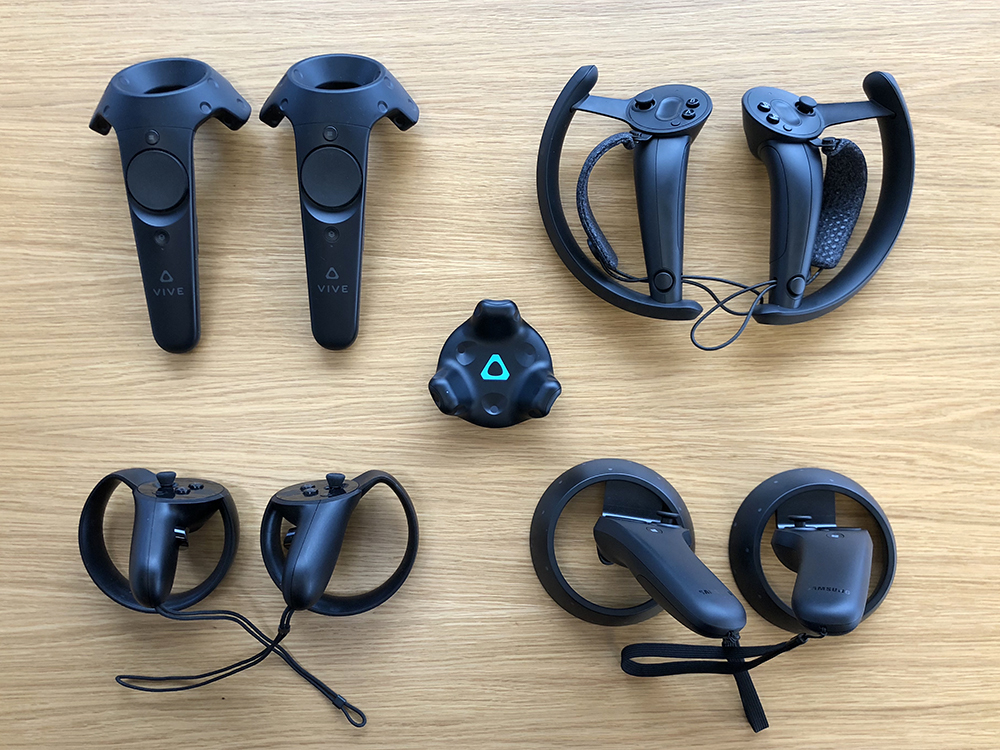
\includegraphics[width=10cm]{figures/introduction/vr_controllers.jpg}%
	\caption[Collection of VR controllers]{A collection of different \ac{VR} controllers. From left to right, top to bottom: HTC VIVE Controllers, Valve Index Controllers (\enquote{Knuckles}), VIVE Tracker, Oculus Touch Controllers, Samsung Odyssey Controllers~\cite{Yang.2018}.}\label{fig:vr-controllers}
\end{figure}

Mapping the movement of our real hands to the virtual world is a common strategy in current \ac{VR} hardware. Not only does it enhance the virtual presence by showing the user a representation of his body, but it also gives the user a natural way of controlling and interacting with the virtual world.

The Leap Motion\footnote{The Leap Motion controller is a hand tracking device, which is often used to display a hand avatar. Website: \href{https://www.leapmotion.com/}{www.leapmotion.com}} sensor uses multiple infrared cameras to track hand poses, which is only possible in front of the sensor. Newer generations of \ac{VR} controllers try to achieve a similar effect with different methods: The Oculus Touch\footnote{The Oculus Touch controllers are hand tracking devices included with the Oculus Rift \ac{HMD}. Website: \href{https://www.oculus.com/rift/}{www.oculus.com/rift}} controllers track the distance of the fingers from the controller and the Valve Index\footnote{The Valve Index is a \ac{HMD} which includes its own set of controllers, called \enquote{Knuckles}. Website: \href{https://store.steampowered.com/valveindex}{store.steampowered.com/valveindex}} controllers even have pressure sensors built-in.

However, for many interactions, hand inspired controllers are not ideal. This applies especially to productive \ac{VR} applications, which require interactions like inputting text for labeling or manipulating \ac{3D} shapes. Most \ac{VR} controllers also require complex external tracking systems.

The Google Cardboard\footnote{The Google Cardboard is a \ac{HMD} made out of cardboard, which uses a smartphone as a display and for tracking. Website: \href{https://vr.google.com/cardboard/}{vr.google.com/cardboard}} uses a smartphone as a display and as a tracking device. This demonstrates the versatility of smartphones. Most people already have one, since they are portable general-purpose devices and are not very expensive anymore. Thanks to \ac{WLAN} and Bluetooth\footnote{Bluetooth is a wireless standard for exchanging data over short ranges between mobile devices.} it is easy to connect the smartphone to other devices.

Smartphones have input devices like buttons, a touch screen, an \ac{IMU}\footnote{An IMU is an electronic component which is part of most smartphones and allows to measure a specific force, angular rate, and magnetic field.}. But also, output devices like the display, vibration motors and speakers are present. This makes them similar to \ac{VR} controllers.

One significant difference between smartphones and common \ac{VR} controllers is that smartphones are not capable of accurate positional tracking. The position can be estimated using the data of an \ac{IMU}, but since the error accumulates over time~\cite[44]{Steed.2013}, this method cannot be used. Additional tracking methods, like using the \ac{WLAN} signal strength, can be used to correct the drift~\cite{Zhang.2015}. However, those methods are still not good enough, because \ac{VR} requires very accurate tracking with short distances.
Besides the missing positional tracking, the other advantages lead to the assumption that the smartphone can be used as an alternative \ac{VR} controller.


\section{Problem Statement}\label{section:problem-statement}
This thesis aims to explore the possibilities of using the smartphone as an interaction device in \ac{VR} experiences. The fundamental question is, whether smartphones are useable as \ac{VR} input devices.

To answer that question, some promising typical \ac{VR} interaction methods have to be implemented using a smartphone. The goal of those experiments is not to create a better system, but rather show that the smartphone can be used as well as common \ac{VR} controllers for specific interactions.

To benchmark the performance, a user study should be performed where participants complete tasks using the prosed input systems.
The performance of the users in those tasks should be evaluated and, if possible, compared with similar methods from other research.

Additionally, a \ac{SUS} user study should be performed to get an assessment of the user's feel for the interface.
\ac{UBII} architecture should be used to implement an abstracted and reusable system.


\section{Outline}\label{section:outline}
In the next chapter, different input methods using a smartphone or similar device from previous research is highlighted. The \ac{UBII} components and architecture, as well as the web-based technology stack used in this project, is then introduced and broken down. Afterward, different methods of using the smartphone as an alternative input device for typical \ac{VR} interactions are going to be introduced. In the fifth chapter, tasks to benchmark the user's performance are then described. The user study and its results are presented afterward. Following the evaluation of the user study results, a final conclusion is drawn.
% !TeX root = ../main.tex
\chapter{Related Work}\label{chapter:related-work}


% ModControl – Mobile Phones as a Versatile Interaction Device for Large Screen Applications
%\section{Mobile Phones as a Versatile Interaction Device for Large Screen Applications}\label{section:mobile-phones-interaction-device-large-screen}
\section{Deller et al.\@}\label{section:deller-2011}
\citeauthor{Deller.2011} propose a modular framework to enable multi-user interactions between smartphones and large-screen applications. A typical client-server architecture with an XML\footnote{XML is a standardized data exchange format that uses human-readable text.}-based protocol is used. They differentiate between application clients (the large screen) and interaction clients (the smartphones)~\cite{Deller.2011}.

The client app is provided with different modules. Some modules offer similar functionality to the experiments implemented in this thesis: Their text module enables users to enter a text while their accelerometer and magnetometer module sends \gls{IMU} data like acceleration and magnetic field data in the background to the server. They also described how they integrated their framework in an application where users can navigate a map and toggle display settings~\cite{Deller.2011}.

The approach presented in this thesis uses a comparable client-server architecture. Also, the modularized abstraction structure is similar to the \enquote{Interactions} of the \gls{UBII} framework used in the experiments of this thesis.


% Phone-based motion control in VR (Klinker)
%\section{Phone-based Motion Control in VR}\label{section:phone-based-motion-control-vr}
\section{Benzina et al.\@}\label{section:benzina-2011}
\citeauthor{Benzina.2011} introduce a system for flying through \glspl{VE} by using a smartphone as input device.
% Since the sight is occluded by the \gls{HMD}, the phone display cannot be used to display information.
They try to find convenient mappings between the users' actions with the mobile phone and the subsequent reactions in the \gls{VE}. To solve this, they investigate the \glspl{DOF} required to implement a quickly learnable and comfortable travel task.

Different methods using the accelerometer, magnetic field sensor, and touch screen for controlling the flight movement are presented and evaluated. They concluded that the most accurate method for controlling the flight uses an approach where an airplane metaphor (four \glspl{DOF}) is simulated~\cite{Benzina.2011}.

\citeauthor{Benzina.2011} use the orientational and the touch screen data, the phone provides, to control a \gls{VE}, as is done in this thesis.


% Mobile Devices for Interaction in Immersive Virtual Environments
%\section{Mobile Devices for Interaction in Immersive Virtual Environments}\label{section:mobile-devices-interaction-ve}
\section{Dias et al.\@}\label{section:dias-2018}
\citeauthor{Dias.2018} propose a solution where the smartphone has a visual representation in \gls{VR}. The visual representation displays information and a \gls{UI} on its virtual screen. The camera in the smartphone tracks a marker on the \gls{HMD} to track its own position relative to the headset. The setup is shown in Figure~\ref{fig:dias-2018}.

\begin{figure}[H]
	\centering
	\begin{subfigure}[t]{0.48\textwidth}%
		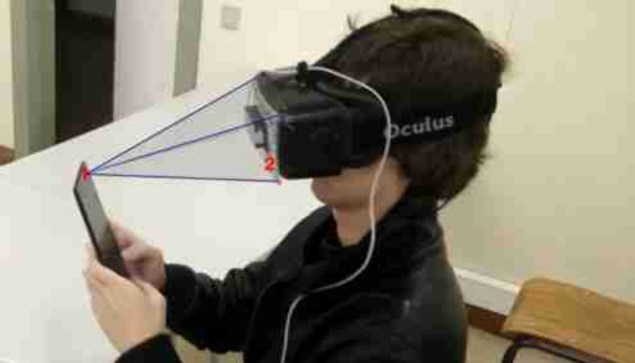
\includegraphics[width=\textwidth]{figures/related_work/dias_2018_tracking.png}
    \caption{The front camera of the smartphone tracks the marker on the \gls{HMD}.
    \newline{}
    Source:~\cite[Figure 3]{Dias.2018}
    }\label{fig:dias-2018-tracking}% chktex 9 % chktex 10
	\end{subfigure}%
	\hspace{0.04\textwidth}%
	\begin{subfigure}[t]{0.48\textwidth}%
		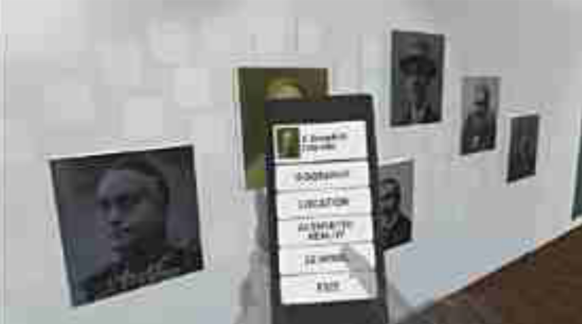
\includegraphics[width=\textwidth]{figures/related_work/dias_2018_virtual_smartphone.png}
    \caption{The virtual smartphone representation and hand avatar in the \gls{VE} while interacting with the \gls{UI}.
    \newline{}
    Source: Adapted from~\cite[Figure 5]{Dias.2018}
    }\label{fig:dias-2018-virtual-smartphone}
	\end{subfigure}%
	\caption[Tracking setup by Dias et al.\@]{The tracking system by \citeauthor{Dias.2018}~\protect\cite[4,5]{Dias.2018}.}\label{fig:dias-2018}
\end{figure}

Because users interact with the \gls{UI} using the touch screen of the smartphone as they would do in real life, the fingers have to be tracked and visualized. Otherwise, users would not know where their fingers are going to hit the touch screen because the sight is occluded physically by the \gls{HMD}. To solve this problem, they attach a Leap Motion sensor to the \gls{HMD} which tracks the fingers to display a hand avatar~\cite{Dias.2018}.

Almost the same research team (\citeauthor{Afonso.2017}) evaluated a selection task using a tablet as an input device in \gls{VR} using the same \gls{VR} setup. They compare the selection time of users selecting a button on the tablet using a realistic hand avatar, a translucent hand avatar, and without any avatar of the hand. Surprisingly, the evaluation shows that users performed the best without any virtual avatar. The authors explain that this is due to the tracking inaccuracies of the tablet and the hand. However, users made fewer selection errors when an avatar was displayed~\cite[247-248]{Afonso.2017}.

Those papers are especially useful for the research of this thesis because they introduce a visual representation of the smartphone in \gls{VR}, which is used in this thesis too. 


\section{Katzakis et al.\@}\label{section:katzakis-2010}
An application to view three-dimensional models controlled with a smartphone was implemented by \citeauthor{Katzakis.2010}. Their approach uses a smartphone to rotate a model which is displayed on a conventional display~\cite[139]{Katzakis.2010}. 

The phone is wirelessly connected to a computer where the model is rendered. The orientation data is provided by the \gls{IMU} of the smartphone and, once calibrated to the screen position, is directly mapped to the model, as seen in Figure~\ref{fig:katzakis-2010}~\cite[139]{Katzakis.2010}. 

\begin{figure}[H]%
  \centering%
  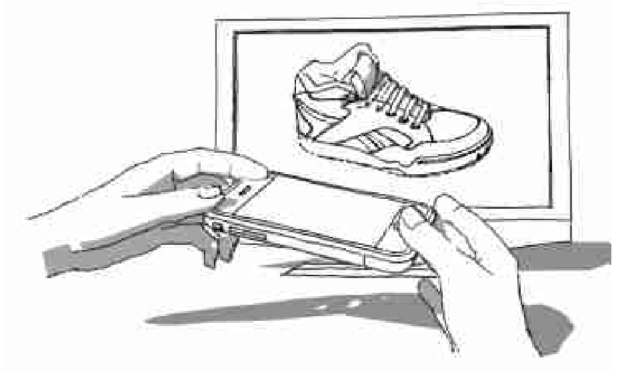
\includegraphics[height=6cm]{figures/related_work/katzakis_2010_3d_object.png}%
  \caption[Model viewer implementation by Katzakis et al.\@]{
  The model viewer implementation by \citeauthor{Katzakis.2010}. The smartphone can be rotated to change the orientation of the three-dimensional model on the display.
  \newline{}
  Source:~\cite[Figure 1]{Katzakis.2010}}\label{fig:katzakis-2010}
\end{figure}

In the evaluation of their system, a mouse, a touch pen, and the smartphone were compared. The latter wins in terms of the time it takes to rotate the model to a certain pose~\cite[140]{Katzakis.2010}.

A similar system, but in use with \gls{VR}, is used in the model viewer experiment presented in this thesis.

\section{Pietroszek et al.\@}\label{section:pietroszek-2014}
\citeauthor{Pietroszek.2014} developed a system called \enquote{Smartcasting}, which allows multiple users to interact with 3D content on a large display using their personal smartphone. They try to explore whether a smartphone can be used as an effective three-dimensional input device for large displays~\cite[119]{Pietroszek.2014}.

The approach uses the orientation from the smartphone to cast a ray into the direction the phone is pointing. A fixed position is used as the origin of the ray as shown in Figure~\ref{fig:pietroszek-2014}, since no positional tracking is available. Objects colliding with the ray can be selected. The depth can be adjusted using the touch screen of the smartphone, to select objects in the three-dimensional world at different depths. The ray and a depth marker are visualized on the display~\cite[121]{Pietroszek.2014}.

\begin{figure}[H]%
  \centering%
  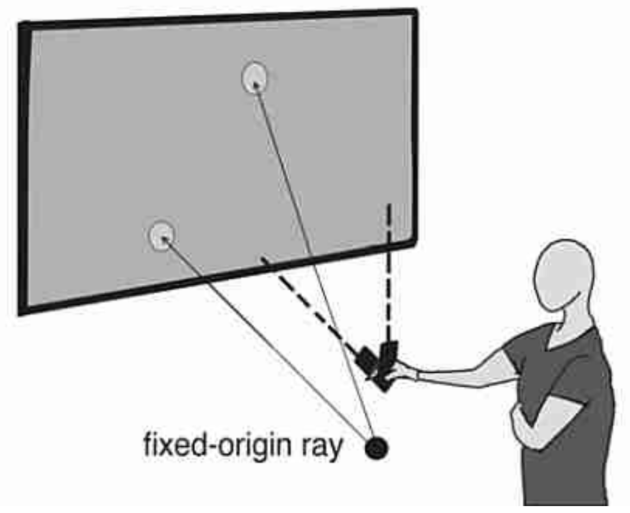
\includegraphics[height=6cm]{figures/related_work/pietroszek_2014_laser_pointer.png}%
  \caption[Laser pointer implementation by Pietroszek et al.\@]{
  The laser pointer interaction with a large display by \citeauthor{Pietroszek.2014}. Since the location of the smartphone is not known, the ray origin is set to a fixed position.
  \newline{}
  Source:~\cite[Figure 3]{Pietroszek.2014}}\label{fig:pietroszek-2014}
\end{figure}

To demonstrate the capabilities of the system, three-dimensional objects in the scene can be positioned and orientated using the laser pointer. Finally, they conducted a study where they compare their system against a Wii controller. The results show no significant difference between those two input methods~\cite[125]{Pietroszek.2014}.

The ray casting system with the fixed-origin ray is also implemented in the laser pointer experiment presented later in this thesis.%, but to select objects in a \gls{VE} from \gls{VR}.


% Design and Implementation of an Immersive Virtual Reality System based on a Smartphone Platform
%\section{Design and Implementation of an Immersive VR System based on a Smartphone Platform}\label{section:design-implementation-vr-system-smartphone-platform}
\section{Steed et al.\@}\label{section:steed-2013}
The approach by \citeauthor{Steed.2013} used a smartphone and a \gls{VR} headset as well as a visual representation of the phone. However, since they do not have positional tracking for the smartphone, the position is fixed relative to the position of the \gls{HMD}. There are two different possible positions, one in front of the users head (shown in Figure~\ref{fig:steed-2013-laser-pointer}) and the other one in front of the users belly (shown in Figure~\ref{fig:steed-2013-ui}). The position switches if a hand raise gesture with the phone in the hand is detected. Gestures and orientation of the smartphone are detected using the data of the \gls{IMU}.

\begin{figure}[H]
	\centering
	\begin{subfigure}[t]{0.45\textwidth}%
		\centering%
		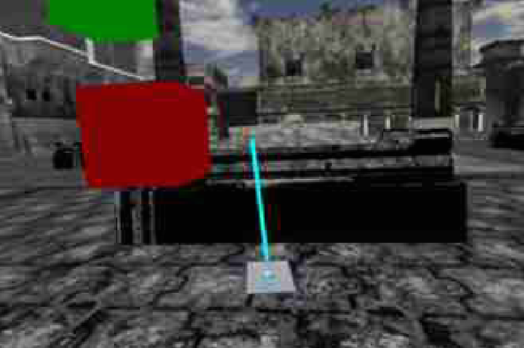
\includegraphics[height=4cm]{figures/related_work/steed_2013_laser_pointer.png}
		\caption{The virtual device in selection mode.}\label{fig:steed-2013-laser-pointer}% chktex 9 % chktex 10
	\end{subfigure}%
	\hspace{0.1\textwidth}%
	\begin{subfigure}[t]{0.45\textwidth}%
		\centering%
		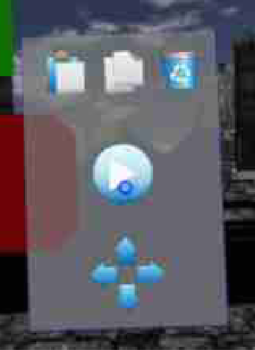
\includegraphics[height=4cm]{figures/related_work/steed_2013_ui.png}
		\caption{The virtual \gls{UI} with the cursor.}\label{fig:steed-2013-ui}
	\end{subfigure}%
  \caption[Virtual smartphone representation by Steed et al.\@]{The virtual smartphone representation by \citeauthor{Steed.2013}.
  \newline{}
  Source: Adapted from~\protect\cite[Figure 1]{Steed.2013}
  }\label{fig:steed-2013}
\end{figure}

On the virtual phone screen, a \gls{UI} is displayed as seen in Figure~\ref{fig:steed-2013-ui}. This \gls{UI} has control elements like buttons, which amongst others, can be used to toggle a selection mode. In the selection mode, the phone casts a ray out of the top (similar to a laser pointer) as seen in Figure~\ref{fig:steed-2013-laser-pointer}. The ray direction can be changed by rotating the smartphone. As soon as a \gls{UI}-button is pressed, the objects intersecting with the ray are selected~\cite{Steed.2013}.

A similar selection approach is implemented in the laser pointer experiment of this thesis. The selection cursor and the fixed phone position also inspired the experiments presented in this thesis.


\section{Markussen et al.\@}\label{section:markussen-2013}
In {\citetitle{Markussen.2013}} \citeauthor{Markussen.2013} explore three different mid-air text input methods for large displays. Mid-air approaches track the users' hands and display a cursor on a external display. This method requires little to no visual attention of the users on their hands, because all the visual feedback is displayed on the large display. With common touch surfaces or displays, visual attention is required because the user has to aim for a virtual button or \gls{UI} element displayed on the touch device.
This approach also allows typing without restricting the users' movement around the display since the user does not have to touch any physical device~\cite[401]{Markussen.2013}.

The first approach, the \enquote{H4 Mid-Air} text entry method, allows to type using four buttons on a physical game controller. To type a character, a specific sequence of the four buttons has to be pressed in the correct order~\cite[406]{Markussen.2013}.

They also propose a reduced keyboard with nine buttons, where three to four characters are combined on one key (called the \enquote{MultiTap} approach). The user moves the cursor by moving his hand, which is tracked by a tracking system. When the cursor hovers over a key, the key is highlighted in orange -- the background of the key changes to red, when a key is activated. To type a character, the user taps a key multiple times in a certain time frame. The number of taps corresponds to the character's index on the key~\cite[407]{Markussen.2013}. % chktex 8

Their final method \enquote{Projected QWERTY} shown in Figure~\ref{fig:markussen-2013} uses a QWERTY\footnote{The name QWERTY describes the US layout for computer keyboards.} keyboard. It uses a similar cursor and highlighting as in the \enquote{MultiTap} approach, but only one tap is required to type a character. To determine the position of the cursor, the hand's position is projected onto the display plane. This makes the cursor movement, relative to hand movement, independent of the distance from the hand to the display~\cite[408]{Markussen.2013}. 

\begin{figure}[H]%
	\centering%
	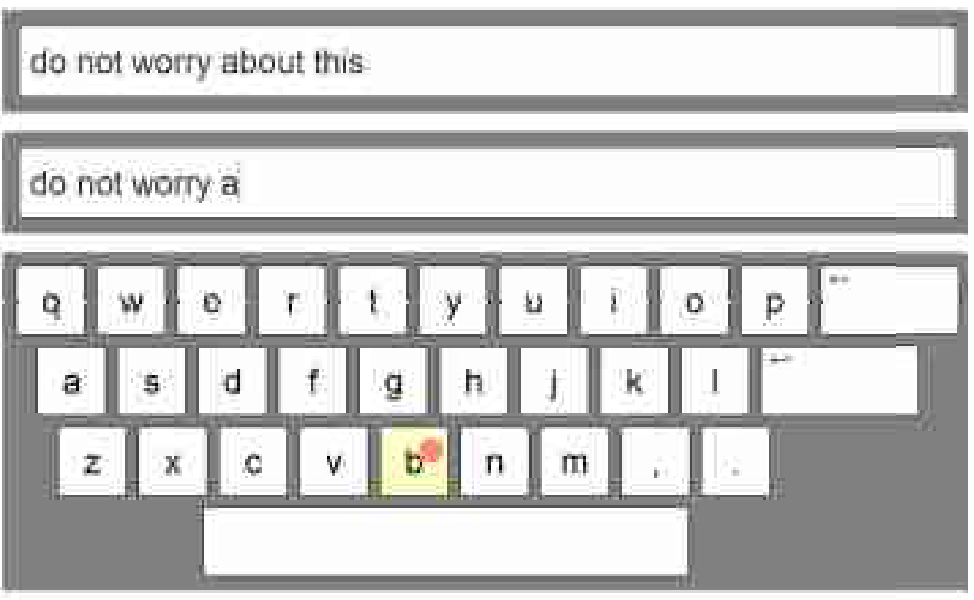
\includegraphics[height=6cm]{figures/related_work/markussen_2013_keyboard.png}%
  \caption[Virtual keyboard implementation by Markussen et al.\@]{
  The virtual keyboard of the user interface from the approach of \citeauthor{Markussen.2013}.
  \newline{}
  Source:~\cite[Figure 5]{Markussen.2013}}\label{fig:markussen-2013}
\end{figure}

A similar visibility-independent text entry method is used in this thesis to demonstrate a text input task for \gls{VR}.

% !TeX root = ../../main.tex
\chapter{Implementation}\label{chapter:implementation}

% !TeX root = ../../main.tex
\section{Ubi-Interact}\label{section:ubi-interact}
\setcounter{footnote}{0} % for some reason, the footnote wants to start at 2

\ac{UBII}\footnote{UBII is currently developed and maintained by Sandro Weber, who is also the advisor for this thesis.} is a framework for distributed applications, which enables to connect all kinds of different devices together. A centralized server is used to manage the system in a local network. The abstraction into devices, topics, and interactions allows decoupling  the implementation of software from device-specific environments.


\subsection{Architecture}\label{subsection:architecture}

The main components of the \ac{UBII} framework are:
\begin{description}
	\item[\ac{UBII} Clients] describe a basic network participant. For every \ac{UBII} client registered on the server also exists one network socket address. Clients are an abstraction of a physical network device. They are defined by a \ac{UID}. 
	\item[\ac{UBII} Devices] can be registered by clients. A \ac{UBII}-device groups different input and output \ac{UBII} devices together. It is defined by a \ac{UID} and a list of \ac{UBII} components.
  \item[\ac{UBII} Components] contain the \ac{UBII} topic name, \ac{UBII} message formats for input/output \ac{UBII} devices and whether it publishes input or receives output data. A data source for such an input \ac{UBII} device, could be any sensor, for example, a button or a camera. Data output examples for input \ac{UBII} devices are lamps and displays.
  \item[\ac{UBII} Message Formats] define the format of data published to a \ac{UBII} topic. Even though it is possible to implement custom ones, most common data types are available. For example, \lstinline[mathescape=true]{Vector4$\times$4} (a four by four matrix), \lstinline{Vector2} (a two-dimensional vector) or \lstinline{boolean} (a binary value) are built-in. % chktex 46
	\item[\ac{UBII} Topics] are data channels which are addressed by a name. \ac{UBII} Clients can publish messages to \ac{UBII} topics, which are registered by a \ac{UBII} device. They are able to receive messages, after subscribing to a \ac{UBII} topic. Such messages (also called \enquote{\ac{UBII} topic data}) are formatted as JSON\footnote{JSON is a standardized data exchange format, that uses human-readable text. It is often used for web-based data communication~\cite[iii]{ECMAInternational.2017}.}-string, whose structure is defined by the device.
	\item[\ac{UBII} Sessions] operate on the server but can be specified by the \ac{UBII} client. They are defined by a \ac{UID} as well as a list of interactions and \textbf{input/output mappings}. The mappings are defined by a \ac{UBII} message format and \ac{UBII} topic name.
	\item[\ac{UBII} Interactions] are reactive components. They operate on \ac{UBII} topics and are defined by a source code snippet\footnote{Currently only JavaScript is supported as a script language.}. \ac{UBII} Interactions are executed in a fixed interval on the \ac{UBII} server. They can subscribe to \ac{UBII} topics and use the received topic data as input, given an input/output mapping description. The output of the \ac{UBII} interaction is published into another \ac{UBII} topic. It is also possible to keep data to use in future executions (persistent state).
	\item[\ac{UBII} Services] are channels, used to send commands or requests to the \ac{UBII} server. For example, they are used to subscribe to a \ac{UBII} topic or list all available \ac{UBII} topics.
\end{description}

The Figure~\ref{fig:ubii-er} visualizes the relationships of the different components.

\begin{figure}[htpb]
  \centering
  \begin{subfigure}{.5\textwidth}
    \centering
    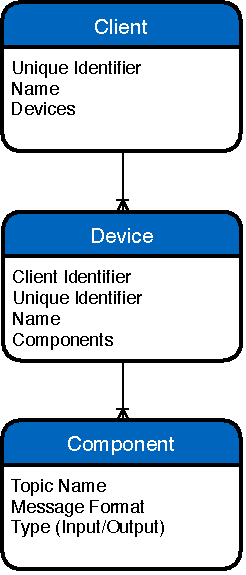
\includegraphics[height=6.5cm]{figures/ubii_er_client.pdf}
    \caption{The client components.}\label{fig:ubii-er-client}
  \end{subfigure}%
  \begin{subfigure}{.5\textwidth}
    \centering
    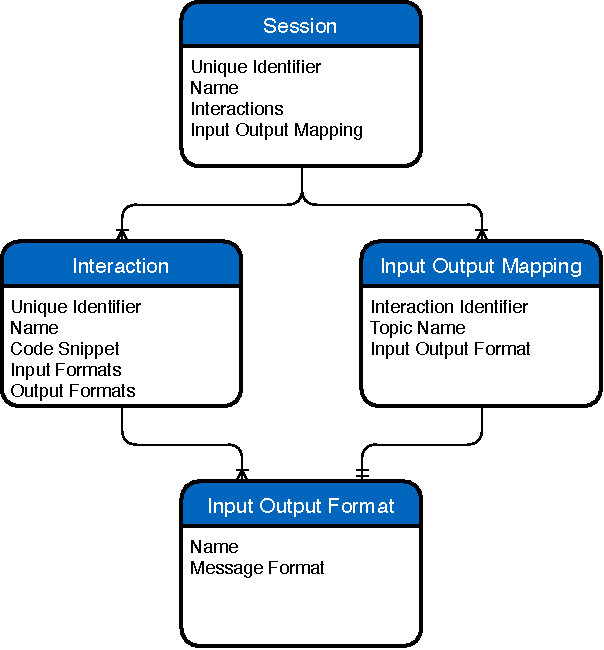
\includegraphics[height=6.5cm]{figures/ubii_er_server.pdf}
    \caption{The session components.}\label{fig:ubii-er-server}
  \end{subfigure}
  \caption[UBII components diagram]{Relationships of the core components in an entity relationship diagram.}\label{fig:ubii-er}
\end{figure}


\subsection{Interactions}\label{subsection:interactions}
A powerful but optional core feature of \ac{UBII} are interactions. As explained in the component overview~(see~\ref{subsection:architecture}), they are reactive components, which operate on \ac{UBII} topics and regularly execute given code snippets (processing functions) on the \ac{UBII} server. Interactions are isolated components, which just depend on topic data and nothing else. This abstraction introduces the possibility to reuse logic in other applications in a similar context. The data flow from a device to the interaction is visualized in the Figure~\ref{fig:ubii-cd}.

\begin{figure}[htpb]
  \centering
  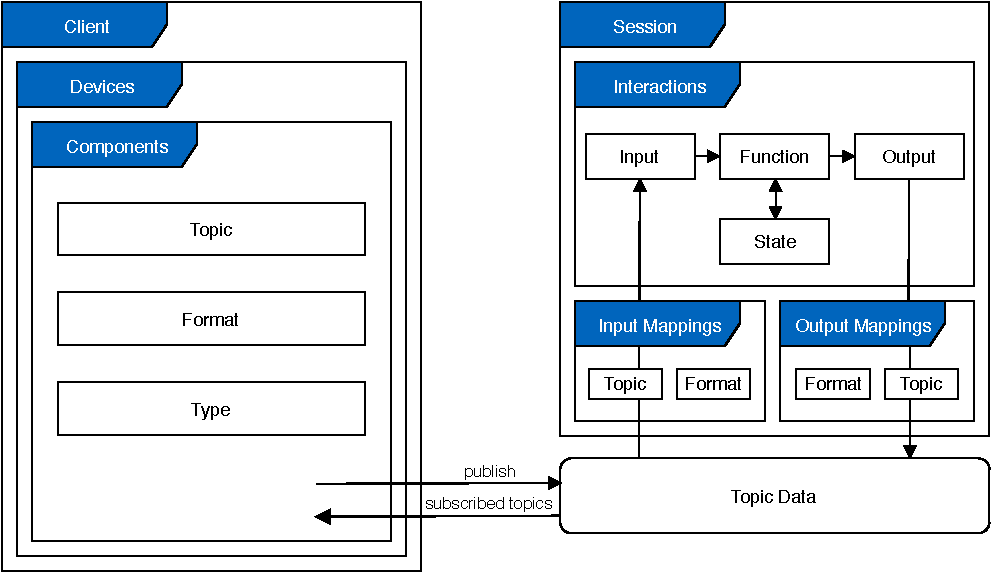
\includegraphics[width=12cm]{figures/ubii_cd.pdf}
  \caption[UBII communication diagram]{\ac{UBII} interaction processing overview. This graphic gives a rough overview of the dataflow when using an \ac{UBII} interaction. Figure created with the help of Sandro Weber.}\label{fig:ubii-cd}
\end{figure}

\ac{UBII} Interactions should be designed generalized so that they are easy to reuse. They can be used to discretize data, converting data to other formats or just to outsource some logic from the application. Concrete examples include detecting button presses, transforming coordinates and evaluating data. An example implementation which detects position changes can be seen in Figure~\ref{fig:ubii-interaction-example}.

% this might be left out or merged into above
They are also useful if two \ac{UBII} topics with different formats should be connected. An example of such a scenario could be an application, which consumes a rotation given in Euler angles. But some input \ac{UBII} devices publish Euler angles in degrees. A \ac{UBII} interaction, which takes Euler angles in degrees from one \ac{UBII} topic and publishes Euler angles in radians to another one could be implemented.

\begin{figure}[H]
  \begin{lstlisting}[language=JavaScript]
    // detect intentional movement by comparing the current position with a previous one
    function (inputs, outputs, state) {
      const threshold = 0.05;

      if (state.position) {
        const vector = {
          x: inputs.position.x - state.lastPosition.x,
          y: inputs.position.y - state.lastPosition.y,
        };
  
        const squaredDistance = Math.pow(vector.x, 2) + Math.pow(vector.y, 2);
  
        outputs.moved = squaredDistance < threshold;
      } else {
        outputs.moved = true;
      }

      state.lastPosition = inputs.position;
    }
  \end{lstlisting}
  \caption[Basic UBII interaction in JavaScript]{An example for an \ac{UBII} interaction written in JavaScript. This \ac{UBII} interaction calculates the squared distance of two points. One of the points is provided through the input, while the other one is stored in the state variable. To achieve this, the Euclidean vector norm of the subtraction of both vectors without the square root is calculated and compared with a threshold constant. The result is then written into the output as a boolean data type. This is used to detect intended changes of the input position.}\label{fig:ubii-interaction-example} %TODO: maybe explain as a formula
\end{figure}

The code snippet has to define a function, which accepts three parameters: 
\lstinline{inputs} is a collection of values, which contains values which were published into a \ac{UBII} topic. The \ac{UBII} topic which was used, is defined by the input mappings of the \ac{UBII} session. \lstinline{outputs} is an empty collection, where values can be added. Those values are then published into a \ac{UBII} topic, defined by the output mappings of the \ac{UBII} session. \lstinline{state} stores a persistent collection of values, which can be used in later executions of the same \ac{UBII} interaction.
% !TeX root = ../../main.tex
% chktex-file 13
\section{Technology Stack}\label{section:technology-stack}

Since most of the existing software for \ac{UBII} was written in \acf{JS}\footnote{\ac{JS} is a just-in-time compiled scripting language, widely used in web technology. It is a dynamic prototype-based language, which supports object-orientated programming~\cite[43, 47]{ECMAInternational.2018}.} using a web-based architecture, I decided to use this approach for my application. This has the major advantage of platform independence. Most modern devices can run web-based software, which means they can also run my application. Also, the application is served by a web server, which means the user does not have to install the software onto his device.

\begin{figure}[htpb]
  \centering
  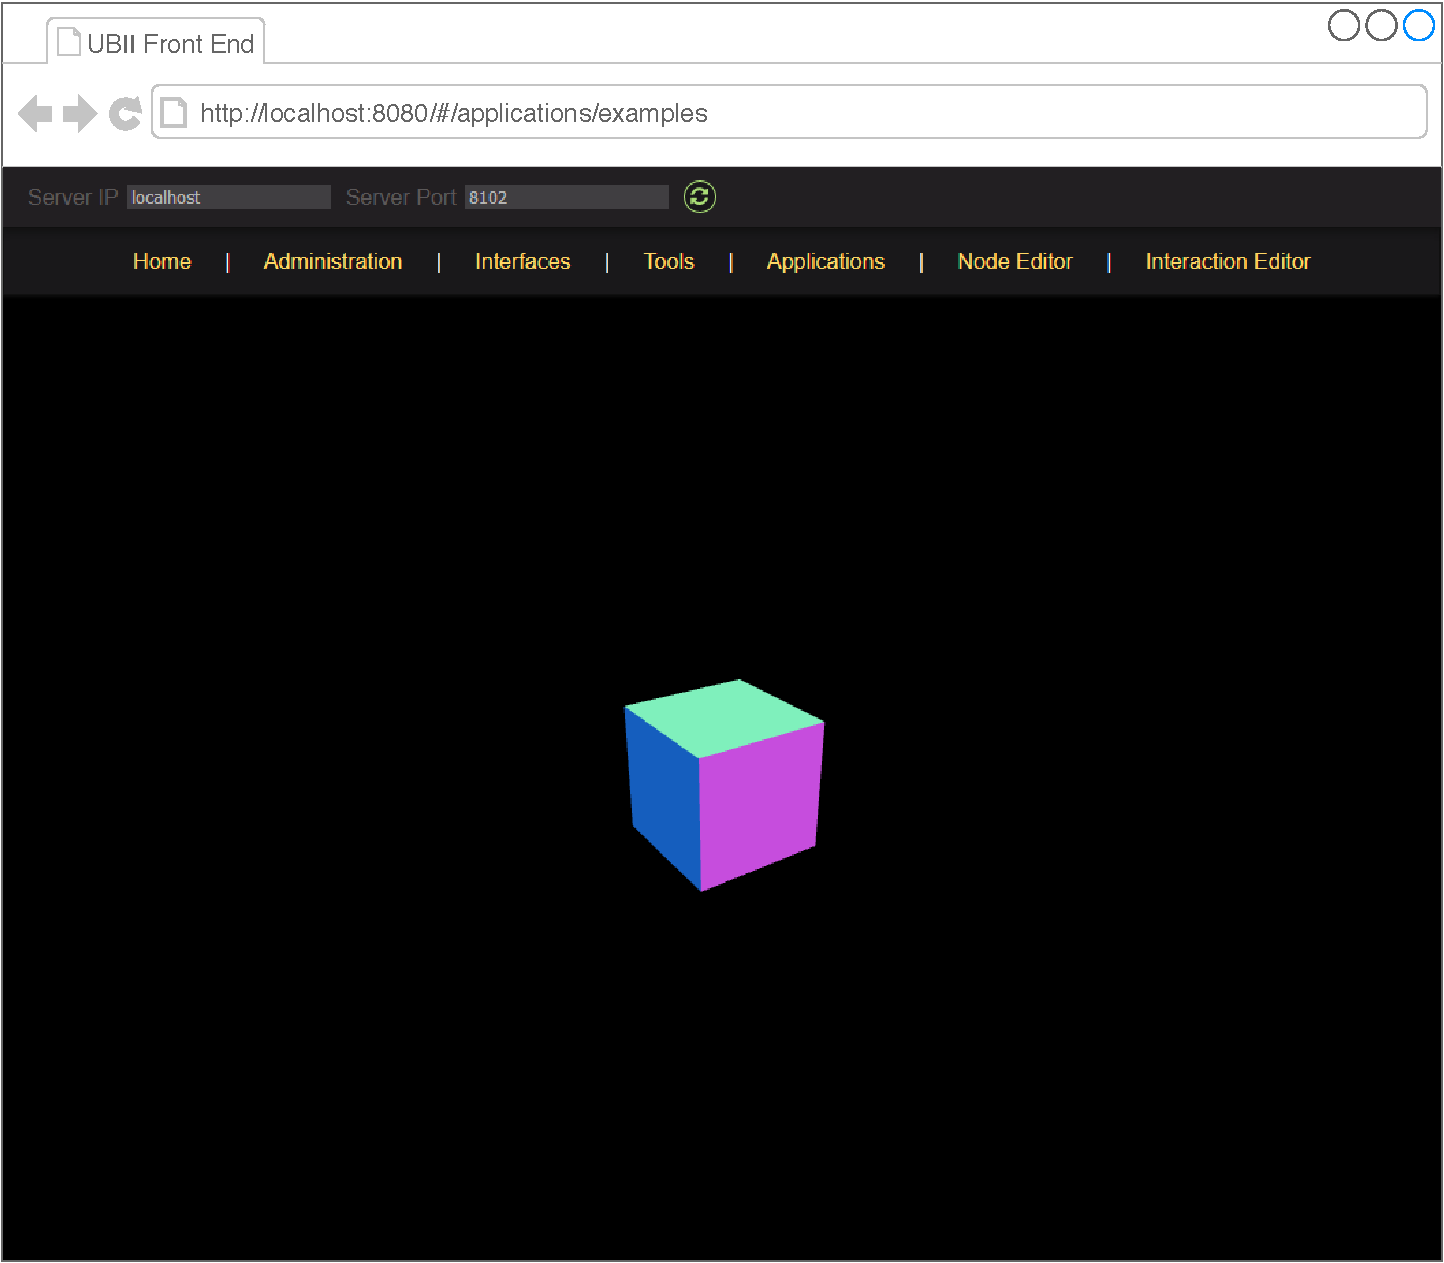
\includegraphics[width=12cm]{figures/ubii_front_end.pdf}
  \caption[Screenshot of the UBII front end]{A screenshot of the UBII front end rendering a 3D cube.}\label{fig:ubii-front-end}
\end{figure}

A web interface with some \ac{UBII} content (the \ac{UBII} front end), demos and debugging tools were already written\footnote{The front end was developed by Sandro Weber, Daniel Dyrda and me.}, so I included my experiments in this application as well. The technology stack of the front end was built with the following technologies:
\begin{description}
  \item[Web APIs] are \acfp{API} available in modern web browsers to provide access to functionality or data outside the browser. The WebAPI is an additional layer of abstraction of the \acp{API} of an operating system. While this has the advantage that the API is the same on every device, this also prevents the access to the raw sensor data\footnote{The specification is available on \href{https://w3c.github.io/deviceorientation/}{www.w3c.github.io/deviceorientation}}. In this thesis, the WebVR \ac{API} and the device orientation \ac{API} were used. The former enables to render to external \ac{VR} headsets. The latter gives access to the data of the \acf{IMU}.
  \item[Vue.js]\footnote{Vue.js: Website: \href{https://vuejs.org/}{www.vuejs.org}; Source~code: \href{https://github.com/vuejs/vue}{www.github.com/vuejs/vue}} is a modern open-source \acl{JS} web framework\footnote{A web framework is a software framework which provides a standard way to build web applications. It comes with tools and libraries to automate and make the development of web applications easier.}~\cite{You.2019}. Being released in 2014 and developed by Evan You, it is a relatively young framework~\cite[17]{Koetsier.2016}. But it quickly gained traction and is quite popular now~\cite[12\psq]{Koetsier.2016}.
  Packages like Vue.js itself, Vue.js plugins and other \acl{JS} libraries are managed using the package manager npm~\footnote{\enquote{NPM} stands for \enquote{Node Package Manager} and is also used in the~\ac{UBII} server itself. Website: \href{https://www.npmjs.com/}{www.npmjs.com}}.
  \item[Three.js]\footnote{Three.js: Website: \href{https://threejs.org/}{www.threejs.org}, Source~code: \href{https://github.com/mrdoob/three.js/}{www.github.com/mrdoob/three.js}} is a lightweight open source library which utilizes WebGL to render \ac{3D} computer graphics~\cite{Cabello.2019}. It can be used to render scenes to the display as well as to a VR headset using WebVR. This high-level library comes with a lot of features, similar to a game engine, like scenes, effects, lights, animation, geometry and much more.
  \item[UBII Client] is an \acl{JS} client for the \ac{UBII} system. It abstracts the protocol and provides high-level functions to register devices as well as send and receive \ac{UBII} topic data. The UBII system uses \acf{Protobuf}\footnote{Protobuf is a mechanism to serialize data. The data is defined in a platform-neutral language, which compiles as a library to all commonly used programming languages~\cite{GoogleLLC.2019b}. Website: \href{https://developers.google.com/protocol-buffers/}{www.developers.google.com/protocol-buffers/}} to serialize the data.
\end{description}

Figure~\ref{fig:ubii-front-end} displays a test view, which uses Vue.js to manage the views and Three.js to render a cube.
% !TeX root = ../../main.tex
\section{Smart Device}\label{section:smart-device}

The \enquote{Smart Device} is a part of the \ac{UBII} front end. It is a general-purpose client, which shares sensor data to different Topics. Because it is web-based, only hardware data which is available through the Web \ac{API} can be obtained. Since it was not designed for a specific use case, it is thought as a general-purpose or testing device. Only touch positions, touch events, orientation, and acceleration are sent to different Topics using the \ac{UBII} Client. For more specific scenarios, the smart device cannot be used, and a custom interface has to be implemented. 

For the experiments in this thesis, though, the smart device client was sufficient, after implementing some improvements. One improvement which was implemented, is a full-screen mode, to prevent unintentional interactions with control elements of the web browser or the operating system. Since the reference system for the orientation, obtained using the Web \ac{API}, is fixed to the earth~\cite[Chapter~4.1]{DevicesandSensorsWorkingGroup.2019}, also a calibration system was implemented. With the press of the \enquote{Calibrate} button, the device is calibrated to the current orientation.


\subsection{Topic Data}\label{subsection:topic-data}

The orientation is provided by the Web \ac{API} through the \lstinline{DeviceOrientation} event. It is defined by three Euler angles named \lstinline{alpha}, \lstinline{beta} and \lstinline{gamma}, as seen in Figure~\ref{fig:webapi-device-orientation}.
While \lstinline{alpha} returns values in the range \(\left[0, 360\right)\), \lstinline{beta} only returns the range \(\left[-180, 180\right)\) and \lstinline{gamma} \(\left[-90, 90\right)\)~\cite[Chapter~4.1]{DevicesandSensorsWorkingGroup.2019}. % chktex 9
This limitation entails that no full orientation tracking is possible with this event. 

\begin{figure}[htpb]
  \centering
  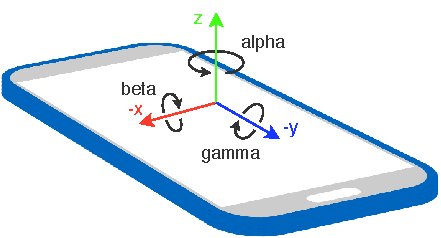
\includegraphics[height=5cm]{figures/implementation/webapi_device_orientation.pdf}
  \caption[Device coordinate system and orientation values]{The specification of the orientation values visualized. The \(x\) and \(y\) axes are inverted for the sake of clarity in this graphic.}\label{fig:webapi-device-orientation}
\end{figure}

The Web \ac{API} also provides the \lstinline{MotionEvent} which returns multiple vectors, one being the acceleration including the gravity (\lstinline{accelerationIncludingGravity}). Since the gravity vector always points to the center of the earth, this vector can be used as a reference vector. Together with the values from the \lstinline{DeviceOrientation} event, the full orientation can be derived. The resulting orientation then has to be further processed because the acceleration vector uses the raw \ac{IMU} acceleration output, which might be very noisy.

The data from the \lstinline{DeviceOrientation} event already provides all three Euler angles and is smoothed. Implementing an algorithm to derive the correct orientation and further process it as the \lstinline{MotionEvent} does, would be outside the scope of this thesis. Because of this consideration, the \lstinline{DeviceOrientation} event data is used in the following experiments.

TThe touch position relative to the display is normalized to floating-point values,  ranging from zero to one. This keeps the data independent of the display resolution and size. Events for starting and stopping touching the screen are sent on different Topics. The acceleration of the smartphone is also sent to a Topic but is not used in any of the experiments of this thesis.


\subsection{UBII Device Definition}\label{subsection:ubii-device-definition}

The smart device is registered as a device in the \ac{UBII} network. The Device definition in \ac{JS} can be seen in Figure~\ref{fig:ubii-device-registration}. The general structure of a Device was described in Chapter~\ref{subsection:architecture}. 

\begin{figure}[htpb]
  \begin{lstlisting}[language=JavaScript]
    const ubiiDevice = {
      name: 'web-interface-smart-device',
      components: [
        {
          topic: clientId + '/web-interface-smart-device/touch_position',
          messageFormat: 'ubii.dataStructure.Vector2',
          ioType: ProtobufLibrary.ubii.devices.Component.IOType.INPUT
        },
        {
          topic: clientId + '/web-interface-smart-device/orientation',
          messageFormat: 'ubii.dataStructure.Vector3',
          ioType: ProtobufLibrary.ubii.devices.Component.IOType.INPUT
        },
        {
          topic: clientId + '/web-interface-smart-device/linear_acceleration',
          messageFormat: 'ubii.dataStructure.Vector3',
          ioType: ProtobufLibrary.ubii.devices.Component.IOType.INPUT
        },
        {
          topic: clientId + '/web-interface-smart-device/touch_events',
          messageFormat: 'ubii.dataStructure.TouchEvent',
          ioType: ProtobufLibrary.ubii.devices.Component.IOType.INPUT
        }
      ]
    };
  \end{lstlisting}
  \caption[Protobuf definition of the smart device]{The smart device definition in JavaScript. It is defined by a name and a list of \ac{UBII} Components. The structure of a Device is further described in Chapter~\ref{subsection:architecture}.}\label{fig:ubii-device-registration}
\end{figure}

A Device and all Topics must be registered with a \ac{UID} for each client because it should be possible to read the data from different devices. This allows for using multiple devices at the same time so that they can be differentiated in Interactions. If the Topic names did not include the \lstinline{clientId}, each connected device would publish to the same Topic, which would make the data unusable.

\begin{figure}[H]
  \begin{lstlisting}[language=Protobuf]
    syntax = "proto3";
    package ubii.dataStructure;
    
    import "proto/topicData/topicDataRecord/dataStructure/vector2.proto";
    
    enum ButtonEventType {
      UP = 0;
      DOWN = 1;
    }

    message TouchEvent {
      ButtonEventType type = 1;
      ubii.dataStructure.Vector2 position = 2;
    }
  \end{lstlisting}
  \caption[Protobuf definition of the touch event]{The definition of the touch event, sent by the smart device client when a user touches or releases the touch screen. It is defined by a position and wether the touch pad was touched or released.}\label{fig:ubii-event-type}
\end{figure}

The touch position is published multiple times per second, but only sends the current position of the first touch on the smartphone display. Using this data, it is not possible to detect whether the display was just touched or released. A new Topic containing a \lstinline{Boolean}-type could have been used, but the position still has to be obtained from the touch position Topic. To not have to check both Topics, the new type \lstinline{TouchEvent} was implemented. The \ac{Protobuf} definition can be seen in Figure~\ref{fig:ubii-event-type}. It contains the two-dimensional position and the binary type \mbox{\lstinline{ButtonEventType},} which can be reused in other events, too. \lstinline{ButtonEventType} is an enumeration type which defines whether the touch interface was just touched or released.

% !TeX root = ../../main.tex
\section{Experiments}\label{section:experiments}

Three experiments were implemented to demonstrate how the smartphone can help with common interactions when using \ac{VR} software.
To achieve consistency amongst all experiments in terms of look and basic functionality, a parent class was implemented. The parent class implements utilities, which are required and inherited by each experiment. It also sets up a basic scene, which contains a skybox, a floor, and lights. Additionally, it handles the connection to the \ac{UBII} Server.


\subsection{Model Viewer}\label{subsection:model-viewer}

\acl{VR} offers a new way of experiencing \ac{3D} content. It is more convenient to view a model from different angles and gives a feel of a real presence of the object. Model viewers like Sketchfab\footnote{Sketchfab is an online platform where one can publish and view \ac{3D} content. Website: \href{https://sketchfab.com}{www.sketchfab.com}} have implemented \ac{VR} support a while ago~\cite{Denoyel.2016}. However, this experience can be enhanced with a smartphone. Models can be rotated without changing the position of the headset or using an expensive hand motion tracking system.

\citeauthor{Katzakis.2010} implemented such a system without using \ac{VR}. His approach uses a smartphone to rotate a model which is displayed on a conventional display. He uses a similar setup as the one presented in this thesis, in which the phone is wirelessly connected to a computer where the model is rendered. The orientation data is provided by the magnetometer and, once calibrated to the screen position, is directly mapped to the model~\cite[139]{Katzakis.2010}. In the evaluation of their system, a mouse, a touch pen, and the smartphone were compared. The latter wins in terms of the time it takes to rotate the model to a certain pose~\cite[140]{Katzakis.2010}.
Since this approach turned out to be very successful, it was used in this experiment as well.

To feature how easy it is to view a more complex model using VR and the smartphone as a manipulator, a human skeleton model is used. This experiment is the only one supporting more than one smartphone client at the same time. For every client that connects, a new skeleton is created. The position is fixed and arranged around the position of the \ac{VR} headset. A scene with multiple connected clients is shown in Figure~\ref{fig:screenshot-exp-mv}.

\begin{figure}[H]
	\centering
	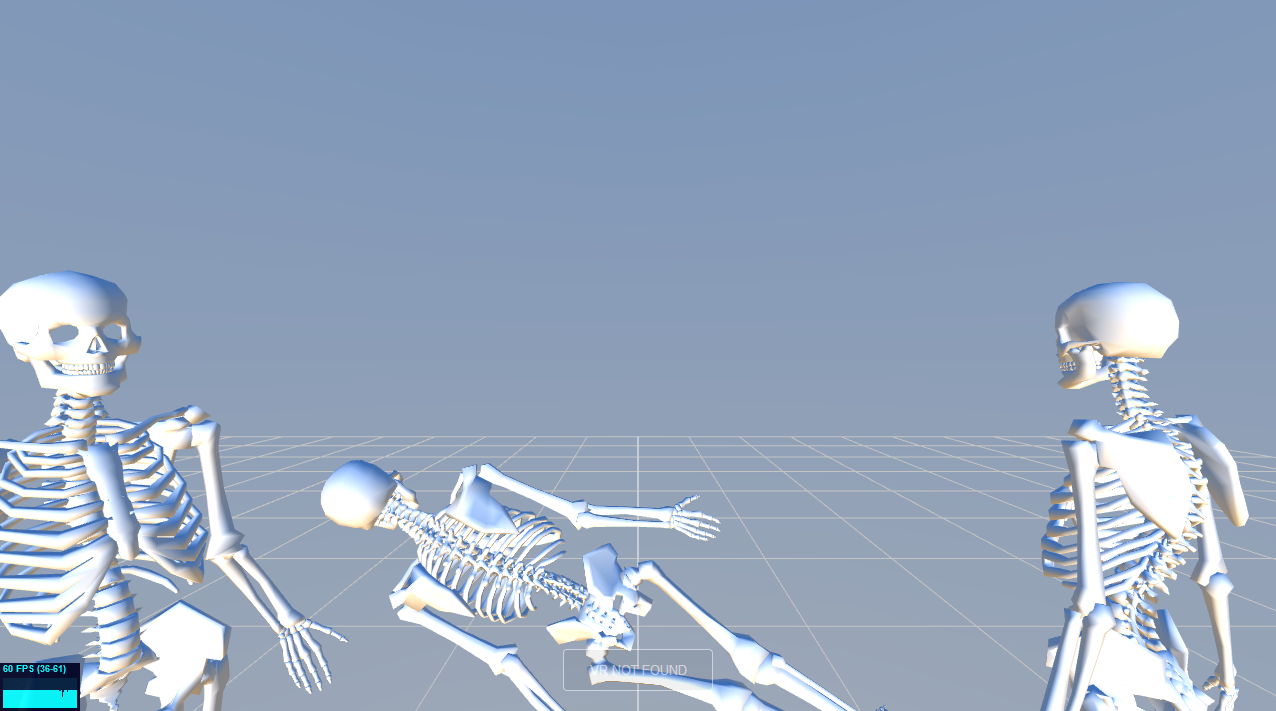
\includegraphics[width=12cm]{figures/implementation/screenshot_exp_mv.png}
	\caption[Screenshot of the model viewer]{A screenshot showing three models, whose rotation is being controlled by three smartphones.}\label{fig:screenshot-exp-mv}
\end{figure}

The experiment always listens for new clients. As soon as one connects, a new Interaction is published, and the resulting Topic subscribed. Since the smart device (see Section~\ref{section:smart-device}) publishes the orientation data in a different format than ThreeJS needs for rendering, a reusable Interaction was created. This Interaction converts the angles from radian to degrees, changes the coordinate system, and publishes them to the \lstinline[breaklines=false]{[client id]/SAVRLaserPointer/orientation} topic. The code for the Interaction is shown in Figure~\ref{fig:ubii-interaction-angles}.

\begin{figure}[H]
	\begin{lstlisting}[language=JavaScript]
  function (input, output, state) {
    if (!input) {
      return;
    }

    const deg2Rad = function(v) {
      return v * Math.PI / 180;
    };

    output.orientation = {
      x: deg2Rad(input.orientation.y),
      y: deg2Rad(input.orientation.x),
      z: deg2Rad(-input.orientation.z)
    };
  }
 \end{lstlisting}
	\caption[A UBII Interaction of model viewer]{This \ac{UBII} Interaction is used to convert the orientation data sent by the smart device to the format ThreeJS needs for rendering. The values are converted by multiplying with an approximate of the number $\Pi$ (\enquote{PI}) and dividing by $180$.}\label{fig:ubii-interaction-angles} %chktex 46
\end{figure}

As in Section~\ref{subsection:topic-data} described, the current implementation does not provide the full angular data needed. This means that the model cannot be rotated upside down, which is very impractical for a model viewing application. However, this can be fixed and is not critical for a proof-of-concept.


\subsection{Laser Pointer}\label{subsection:laser-pointer}

Selecting elements in a virtual world is an essential interaction most \ac{VR} applications use. The selection of elements in a \ac{2D} environment with standard input devices like a mouse or touch screen is rather trivial. However, the selection of elements in a \ac{3D} environment is problematic because the element might be too far away from the user or the cursor.

Ray casting\footnote{Ray casting describes a technique to determine the objects which intersect with a ray, cast from a given point into a given direction.} is used to solve this problem: A ray, with the virtual devices' position as origin, is created. Then, the element first hit by the ray is selected. Implementations without a tracked device, often use the position and orientation of the \ac{HMD}. The ray is fixed to the head of the user and cast along his viewing direction~\cite[23]{Kamm.2018}. This forces the user to keep the head still and look at a particular object to select it until a button is pressed or a specific time has passed.

% TODO: maybe explain some more strategies, like in the keyboard chapter

A better solution is the use of handheld controllers, where the position of the controller is used as origin for the ray. Since the smartphone provides orientation data, it can be used for this task, too. However, most handheld controllers also have positional tracking, which allows them to represent the hand of a user by displaying a virtual phone. This emulates the use of a handheld laser pointer in the real world. Since a smartphone does not have positional tracking, the origin has to be somewhere else.

%\citeauthor{Argelaguet.2013} evaluated more than 30 different selection techniques for virtual environments, but no technique uses the orientation but not the position of the pointing device~\cite[Table 1]{Argelaguet.2013}.
Again, the head could be used, but then the user would have no visual representation of the rotation of the phone. The user has to see where the ray is going, even when rotating it in the opposite direction of the view direction. To give the user a better feel for the direction he is pointing, a visual representation is needed.
To work around the missing position data of the device, the approach by \citeauthor{Pietroszek.2014} is used: The ray origin is set to a fixed location relative to the users head where the phone could be in the real world~\cite[Figure 3]{Pietroszek.2014}.

The ray origin is represented by a \ac{3D} phone model, whose orientation is synchronized with the one from the last connected smart device client (see Section~\ref{section:smart-device}), similar to the first experiment (\ref{subsection:model-viewer}). To keep the virtual phone inside the view frustum of the user, it rotates relative to the user on the up-axis and moves only on the right/forward-axis.
A line is attached to the front of the phone (the \enquote{laser}) to indicate the direction of the ray. A screenshot of this setup can be seen in Figure~\ref{fig:screenshot-exp-lp}.

\begin{figure}[H]
	\centering
	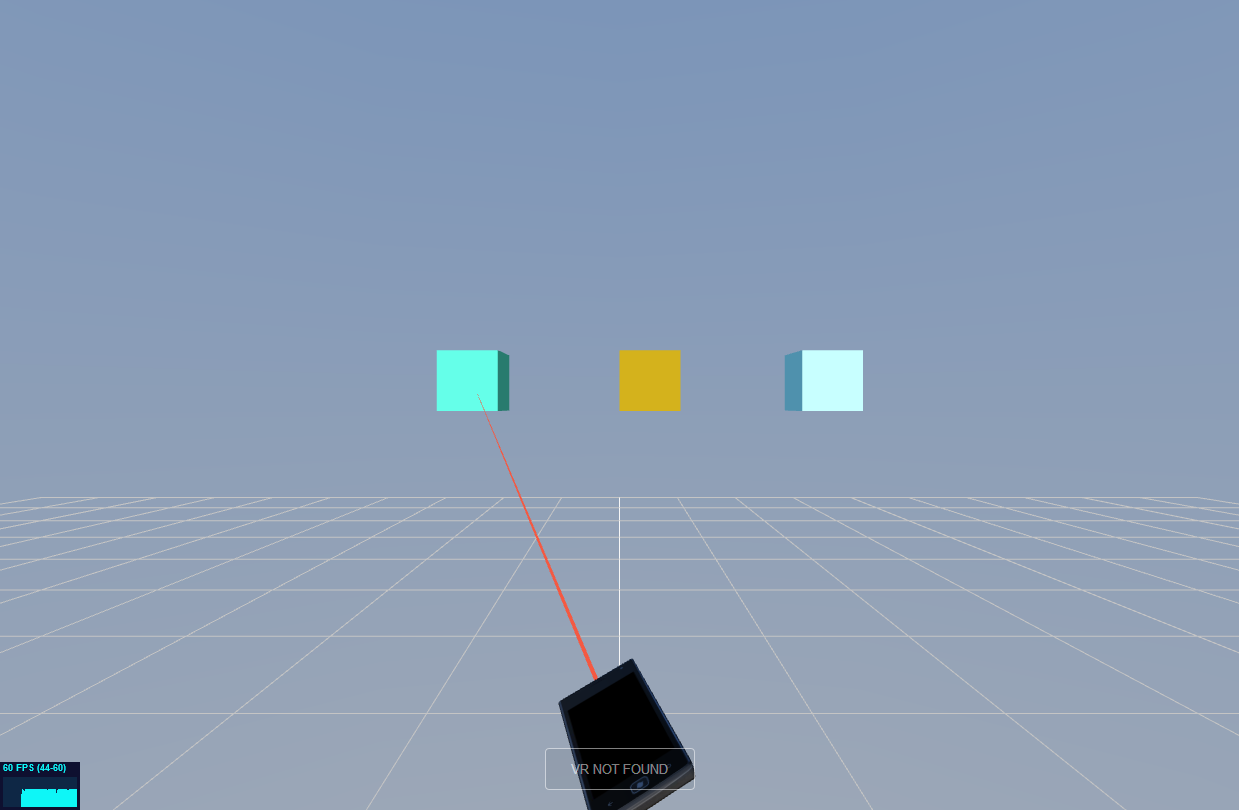
\includegraphics[width=12cm]{figures/implementation/screenshot_exp_lp.png}
	\caption[Screenshot of the laser pointer]{A screenshot of the virtual laser pointer and selectable cubes.}\label{fig:screenshot-exp-lp}
\end{figure}

In addition to the orientation Topic, this implementation subscribes to the touch events Topic. The \lstinline{touch down} event is needed to trigger the actual selection.
To illustrate a selection task with this system, cubes float in front of the user. If he points the laser at one and touches the display, the randomly colored cubes will change their color. This works not only with cubes but with any mesh. Also, the system could trigger any kind of event or action.


\subsection{Virtual Keyboard}\label{subsection:virtual-keyboard}

Text input is not an easy task to perform in \ac{VR}. However, it is often required for labeling, annotation, entering filenames for saving operations, and setting parameters in visualizations and other productive \ac{VR} software~\cite[2154]{Rhoton.2002}. This is why many applications try to avoid it.

Tilt Brush\footnote{Tilt Brush by Google is a tool for three-dimensional painting in VR. Website: \href{https://www.tiltbrush.com/}{www.tiltbrush.com}} avoids this during the select and load process of scenes, by identifying the scenes with a screenshot of the scene rather than a filename. To save a scene, the user gets a virtual camera attached to his hand motion controller, which he then uses to create a thumbnail of the current scene~\cite{GoogleLLC.2019}. % chktex 13

Some applications use a laser pointer either attached to the motion controller or to the \ac{HMD} to select virtual keys on a \ac{2D} image of a keyboard~\cite{WeelcoInc.2017}. A more recent approach is the frequently called \enquote{drum keyboard}, which attaches drum sticks to the hand controllers which are then used to hit \ac{3D} keys~\cite{Weisel.2017}.

Other approaches use hand gloves~\cite{Evans.1999,Rhoton.2002}, a real keyboard~\cite{McGill.2015,Walker.2017} or other peripherals~\cite[111\psq]{Gonzalez.2009}. Also, methods like speech recognition~\cite[2154\psqq]{Rhoton.2002} and handwritten character recognition~\cite[113]{Gonzalez.2009} are possible.

Similar to the approach by~\citeauthor{Dias.2018} to implement user interfaces using a real smartphone and a virtual representation in the \ac{VE}~\cite[5]{Dias.2018}, this experiment uses a virtual keyboard as seen in Figure~\ref{fig:screenshot-exp-vk}.
The surface of the virtual keyboard is mapped to the touchscreen of the smart device (see Section~\ref{section:smart-device}). The cursor, represented by a blue circle, visualizes the position of the finger on the touchscreen.

\begin{figure}[H]
	\centering
	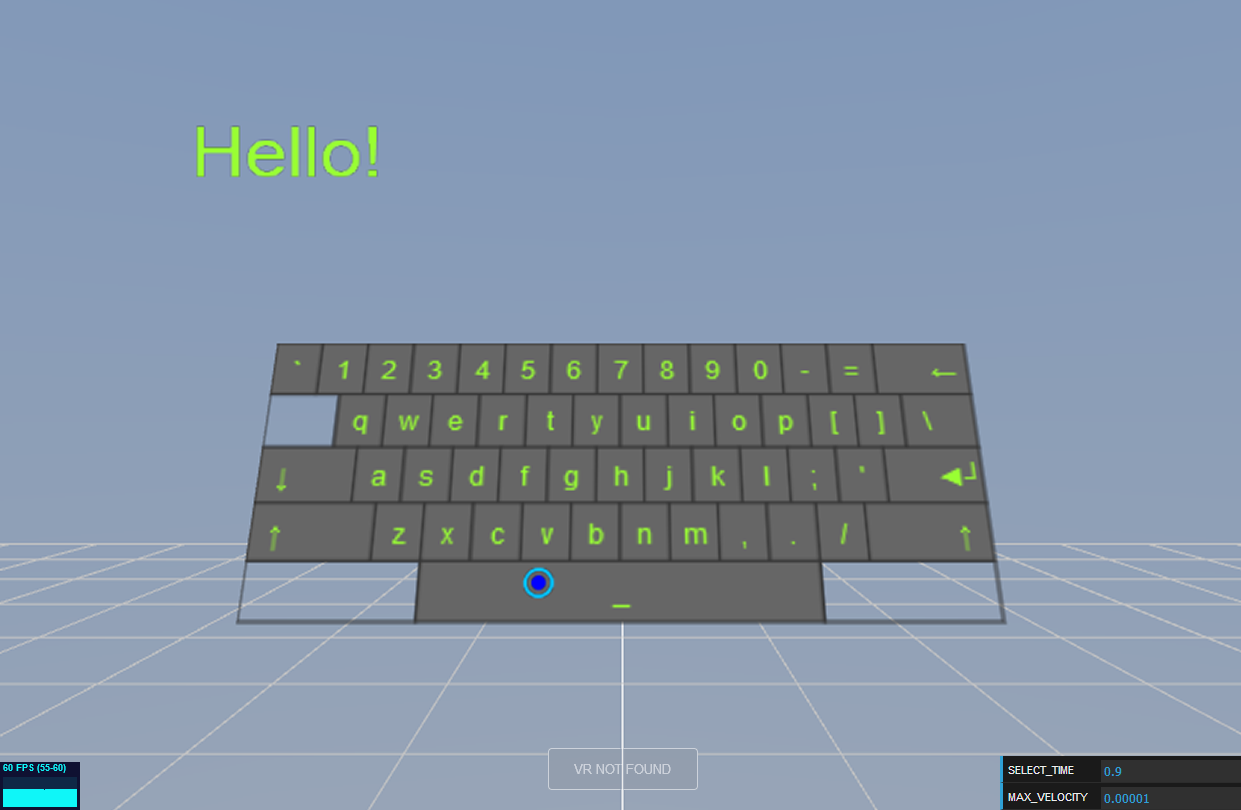
\includegraphics[width=12cm]{figures/implementation/screenshot_exp_vk.png}
	\caption[Screenshot of the virtual keyboard]{A screenshot of the virtual keyboard with the blue cursor and the previously typed text.}\label{fig:screenshot-exp-vk}
\end{figure}

When executing the keypress on the first touch and without a cursor (like a regular smartphone keyboard), the user would not know which key he is going to hit with his finger, because his sight is obscured by the \ac{HMD}. \citeauthor{Dias.2018} work around this problem by using a Leap Motion sensor to visualize the finger positions~\cite[4]{Dias.2018}.

In this implementation, the cursor is only visible when the user is touching the screen. To select a key, the user has to move the cursor on top of a key and then keep the finger there for roughly a second. As long as the user is holding his finger on a key to select it, the blue circle increases in size to display the selection progress.

Three components were implemented as \acl{JS} classes for this experiment. The \lstinline{SmartphoneCursor} component uses the touch events and position data to display a blue circle (the cursor) on a given area in the scene. If the touch screen is touched, the position of the circle is synchronized with the position of the finger on the touch screen.

To detect intentional movements, the current position is subtracted by the position of the previous frame. If the length of the resulting vector is smaller than a specific threshold value, it is assumed that the movement was not intentional. This calculation depends on the current framerate, which is not a good practice because the selection time will be different depending on the current framerate. However, as the target framerate is 60 frames per second, and the testing system does not have issues in reaching this target, it is not a critical problem.

As long as intentional movements are not detected, a timer counts up to a specific value (with the default settings, roughly one second). After reaching the value, a select event containing the cursor position is sent to the main program. To visualize the selection progress, a second blue circle gets larger until it fills up the whole cursor and finally disappears again.

The second component renders a virtual QWERTY\footnote{The name QWERTY describes the US layout for computer keyboards.} keyboard to the scene. The keyboard layout, whose definition is shown in Figure~\ref{fig:virtual-keyboard-layout}, can be adjusted pretty easily. Every key has a character or an action assigned as well as properties which influence the look. Special keys like the caps, caps lock, enter and delete key are fully functional as known from a real keyboard. When caps lock is activated, the key is drawn in blue, and all characters are display in upper case.

\begin{figure}[H]
	\begin{lstlisting}[language=JavaScript]
  // rows
  [
    // columns
    %\dots%
    [ 
      // keys
      %\dots%
      {
        key: '=', // the returned character if no action is present otherwise just a label
        keyCaps: '+' // the returned character if in caps mode 
      },
      {
        key: '%\color{TUMAccentOrange}\textleftarrow%',
        action: KEY_ACTIONS.DELETE_ONE, // a special key action; in this case, it deletes the last character
        width: 2, // with of the key
        align: KEY_ALIGNMENT.RIGHT // the alignment of the label on the key
      }
      %\dots%
    ],
    %\dots%
  ],
  \end{lstlisting}
	\caption[Virtual keyboard layout definition]{The definition of the virtual keyboard layout, written in \ac{JS}. It is defined as a \ac{2D} array, where the first dimension corresponds to the key rows and the second one to the keys column-wise.}\label{fig:virtual-keyboard-layout}
\end{figure}

The \lstinline{VirtualKeyboard} class draws the keyboard by providing it with the keyboard layout, height, and width as input. If the \lstinline{onPress(coordinates)} function is called, for example by the cursor component, the pressed key is calculated and returned using the provided position. The main program then applies the key to a string and sends the result to the third component. % chktex 36

The \lstinline{TextDisplay} component renders a given text inside a given area to a texture. If the text is changed, it automatically updates and redraws the texture.
% !TeX root = ../../main.tex
\chapter{Evaluation}\label{chapter:evaluation}

% !TeX root = ../../main.tex
\section{Overview}\label{section:evaluation-overview}
In order to test the usability of the smartphone as an assistant device for \gls{VR}, a user study was conducted. In the study, participants had to complete three tasks to measure the usability. Also, a \gls{SUS} user study was performed to get feedback from the users.

%The user was given a minute to acclimatize to the experiment, in order to get a feel for the interaction
The procedure of the user study was as follows:
\begin{enumerate}
  \item Introduce the topic to the user
  \item Have the user fill out the consent form
  \item Have the user fill out the preliminary questions
  \item Hand the user the \gls{HMD} and the calibrated smartphone
  \item For each experiment (random order):
  \begin{enumerate}
    \item Brief the user on the experiment
    \item Let the user play around in the experiment for a minute to get a feel for the interaction
    \item Save the anonymized task results
    \item Conduct the \gls{SUS} usability study
  \end{enumerate}
\end{enumerate}

The evaluation was conducted in two different locations at different times of the day. Before starting the study, the \gls{WLAN} connection and network performance were tested and evaluated as appropriate. The specifications of the \gls{PC}, \gls{HMD} and smartphone of the different evaluation setups is listed in the Appendix~\ref{chapter:append-user-eval-devices}. The \gls{PC} was able to run the application with an average of 60 frames per second, which is enough to run a smooth \gls{VR} experience. The \gls{WLAN} connection and devices were capable of 20 Mbps\footnote{Mbps stands for megabits per second. This unit is often used in reference to internet speeds.}, which is enough for synchronizing data without a noticeable lag.

Before starting the experiments, demographic questions had to be answered by the participants. The preliminary questions also asked to rate the use of specific technologies and statements on a Likert scale\footnote{A Likert scale is a type of rating scale which ranges from \enquote{Strongly disagree} to \enquote{Strongly agree.}}. 

After each experiment, a \gls{SUS} survey was conducted. The \gls{SUS} study uses a set of 10 questions, which are rated from strongly disagree (1) to strongly agree (5), to assess the usability of a system~\cite[3]{Brooke.1996}. \citeauthor{Finstad.2006}'s suggestion to change the eighth question to make it more easily understandable for non-native speakers was implemented~\cite[188]{Finstad.2006}, because the study was performed in Germany. The evaluation form, which includes the preliminary questions and \gls{SUS} study, can be found in Appendix~\ref{chapter:append-user-eval-form}.

A final score, ranging from zero to 100, was then calculated from the individual answers~\cite{Brooke.1996}. \citeauthor{Bangor.2009} proposes a grading system for \gls{SUS} scores, which maps a value to a letter of the typical American school grading scale~\cite{Bangor.2009}. This system is used to asses the meaning of the score.

Useful metrics were collected while users performed the tasks. The anonymized metric data contained timing and interaction specific statics. The following statistics were collected:
\begin{enumerate}
  \item Model viewer experiment
  \begin{enumerate}
    \item Count of matched poses
    \item Date and time
  \end{enumerate}

  \item Laser pointer experiment
  \begin{enumerate}
    \item Count of clicks (touched touch screen)
    \item Count of hits (hit a cube)
    \item Date and time
  \end{enumerate}
  
  \item Virtual keyboard experiment
  \begin{enumerate}
    \item Count of backspace presses (undo operations)
    \item Time it took to write the given sentence
    \item Date and time
  \end{enumerate}
\end{enumerate}
The data was saved in the JSON format and downloaded automatically after completing a task.
\section{Results}\label{section:eval-results}

% Commands to edit stats which might change later. 

% demographic questions
\newcommand{\participantsCount}{23}
\newcommand{\participantsMale}{21}
\newcommand{\participantsAge}{23}

% model viewer statistical facts
\newcommand{\evalExpMvAvgPoses}{2.83}
\newcommand{\evalExpMvStdPoses}{1.94}
\newcommand{\evalExpMvParticipants}{\participantsCount}

% avg lp experiments
\newcommand{\kammAvgHits}{36.23/60}
\newcommand{\kammAvgStd}{6.87/60}
\newcommand{\youngAvgHits}{0.85}
\newcommand{\youngAvgStd}{-}
\newcommand{\oursAvgHits}{26.13/30}
\newcommand{\oursAvgStd}{5.52/30}

% model viewer sus scores
\newcommand{\evalExpMvSusScore}{83.04}
\newcommand{\evalExpMvSusGrade}{B}
\newcommand{\evalExpMvSusAdj}{\enquote{Good}}

% model viewer sus scores
\newcommand{\evalExpLpSusScore}{91.41}
\newcommand{\evalExpLpSusGrade}{A}
\newcommand{\evalExpLpSusAdj}{\enquote{Excellent}}

% model viewer sus scores
\newcommand{\evalExpVkSusScore}{71.63}
\newcommand{\evalExpVkSusGrade}{C}
\newcommand{\evalExpVkSusAdj}{\enquote{Ok}}

% Calculations
\newcommand{\participantsFemale}{\pgfmathparse{\participantsCount - \participantsMale}\pgfmathprintnumber[fixed, precision=2]{\pgfmathresult}}%chktex 8 chktex 1

The results were evaluated in Python. Also, the plots were created using several Python libraries.

\participantsCount{} people participated in the evaluation. \participantsMale{} identified as male while the others identified as female. The average age is \participantsAge{} years, so most of participants were relatively young. This could influence the results since younger people might be more exposed to new technologies and therefore, could pick up new technologies faster.
% The evaluation was conducted during different times of the day. does say nothing

The main disciplines and degrees of the participants are shown in Table~\ref{tab:sus-d}. As seen in Table~\ref{tab:sus-degree}, the highest degree of half of the participants is a high school degree or equivalent.
Table~\ref{tab:sus-discipline} exhibits that the disciplines are spread amongst different fields.

\begin{table}[H]
	\centering
	\begin{subtable}{.5\linewidth}
		\footnotesize
		\centering
		\begin{tabular}{l c c}
			\toprule
			Degree             & Count & Percentage \\
			\midrule
			High school degree & 13    & 56.52\%    \\
			Bachelor's degree  & 6     & 26.09\%    \\
			Master's degree    & 2     & 8.70\%     \\
			Diploma's degree   & 1     & 4.35\%     \\
			Approbation        & 1     & 4.35\%     \\
			\bottomrule
		\end{tabular}
		\caption{Bar charts of the answers to question A3: \enquote{What is the highest degree or level of school you have completed?} Most participants' (56.52\%) highest degree is the high school degree. Others (43.48\%) have at least one academic degree.}\label{tab:sus-degree}
	\end{subtable}%
	\begin{subtable}{.5\linewidth}
		\footnotesize
		\centering
		\begin{tabular}{l c c}
			\toprule
			Discipline              & Count & Percentage \\
			\midrule
			Computer Science        & 7     & 30.43\%    \\
			Physics                 & 2     & 8.70\%     \\
			Automation and Robotics & 1     & 4.35\%     \\
			Book Science            & 1     & 4.35\%     \\
			Chemistry               & 1     & 4.35\%     \\
			Computational Biology   & 1     & 4.35\%     \\
			Economics               & 1     & 4.35\%     \\
			Electrical Engineering  & 1     & 4.35\%     \\
			Law                     & 1     & 4.35\%     \\
			Medicine                & 1     & 4.35\%     \\
			Musicology              & 1     & 4.35\%     \\
			Pharmacy                & 1     & 4.35\%     \\
			Public Service          & 1     & 4.35\%     \\
			Statistics              & 1     & 4.35\%     \\
			Technical Engineering   & 1     & 4.35\%     \\
			Technology Management   & 1     & 4.35\%     \\
			\bottomrule
		\end{tabular}
		\caption{Bar charts of the answers to question A4: \enquote{What is your main discipline?} Roughly one third (30.43\%) are computer science students. \participantsCount{} participants stated 16 different disciplines, which is well distributed.}\label{tab:sus-discipline}
	\end{subtable}
	\caption[Degree and discipline of participants]{Bar charts of the highest degree (question A3) and main disciplines (question A4) of the participants.}\label{tab:sus-d}
\end{table}

All participants used their smartphone multiple times a day during the last six months. Most participants (78.26\%) used their computer to work or to study more than once per day during the last six months. 17.39\% state that they used it daily, and only one participant used his computer one to three times a week for work or studies during the last six months.

As seen in Figure~\ref{fig:res-demo-q8-s3}, most participants (60.87\%) played computer games more than three times a month during the last six months. Figure~\ref{fig:res-demo-q8-s4} shows that most participants (91.30\%) used \gls{VR} less than once per month during the last six months. A huge portion (39.13\%) did not use \gls{VR} at all in the last six months.

\begin{figure}[H]
	\centering
	\begin{subfigure}{.48\linewidth}%
		\centering
		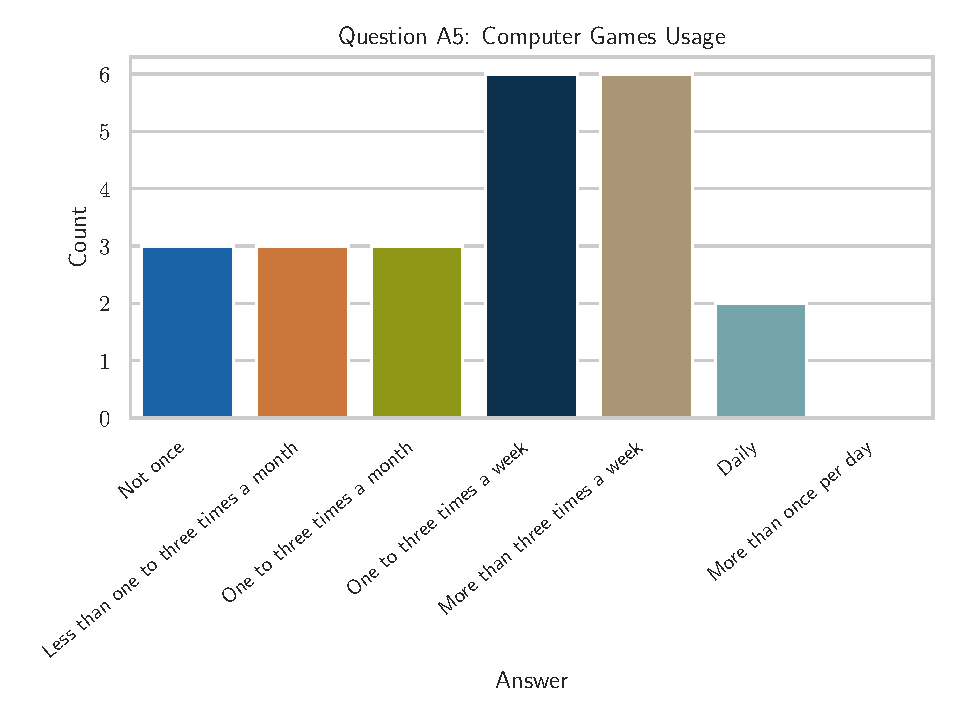
\includegraphics[width=\linewidth]{figures/evaluation/res_demo_q8_s3.pdf}
		\caption{Bar charts of the answers to the question A5: \enquote{Please rate how much you used computer games in the last six months.}}\label{fig:res-demo-q8-s3}
	\end{subfigure}%
	\hspace{0.03\linewidth}
	\begin{subfigure}{.48\linewidth}%
		\centering
		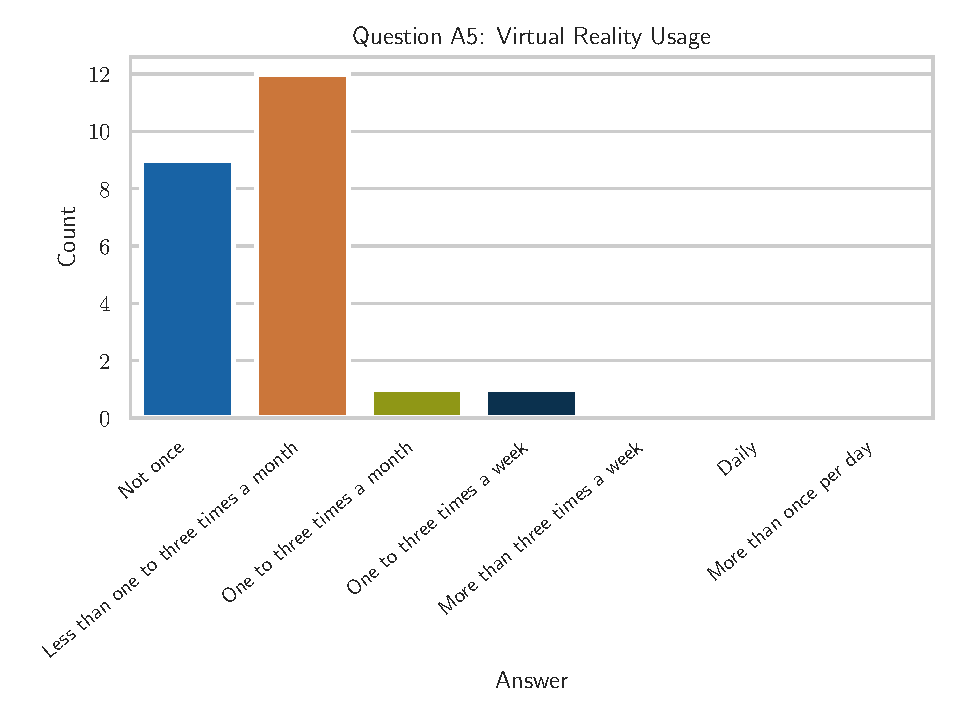
\includegraphics[width=\linewidth]{figures/evaluation/res_demo_q8_s4.pdf}
		\caption{Bar charts of the answers to the question A5: \enquote{Please rate how much you used virtual reality headsets in the last six months.}}\label{fig:res-demo-q8-s4}
	\end{subfigure}%
	\caption[Computer games and VR usage]{Bar charts of the answers to the question A5 about computer games and virtual reality headset usage. While \gls{VR} is used rarely, most survey participants (60.87\%) played computer games more than three times a month during the last six months. None of the participants is using \gls{VR} on a daily basis.}\label{fig:res-demo-q8}
\end{figure}

The participants were asked three questions regarding their experience with \gls{VR}, which could be answered with values ranging from one (\enquote{none}) to five (\enquote{a lot}). The first questions asked about the knowledge the user had of \gls{VR}. As can be seen in the box plots\footnote{The boxes indicate the range from the \nth{25} to the \nth{75} percentile. The bars outside the box (\enquote{whiskers}) indicate the \nth{90} and \nth{10} percentile. The median (\nth{50} percentile) is marked by the line in the center. Outliers are marked with diamond shapes.} in Figure~\ref{fig:res-demo-q9}, the general knowledge about \gls{VR} seems to be rather low (Mean: 2.83; \gls{STD}: 1.03).

\begin{figure}[H]
	\centering
	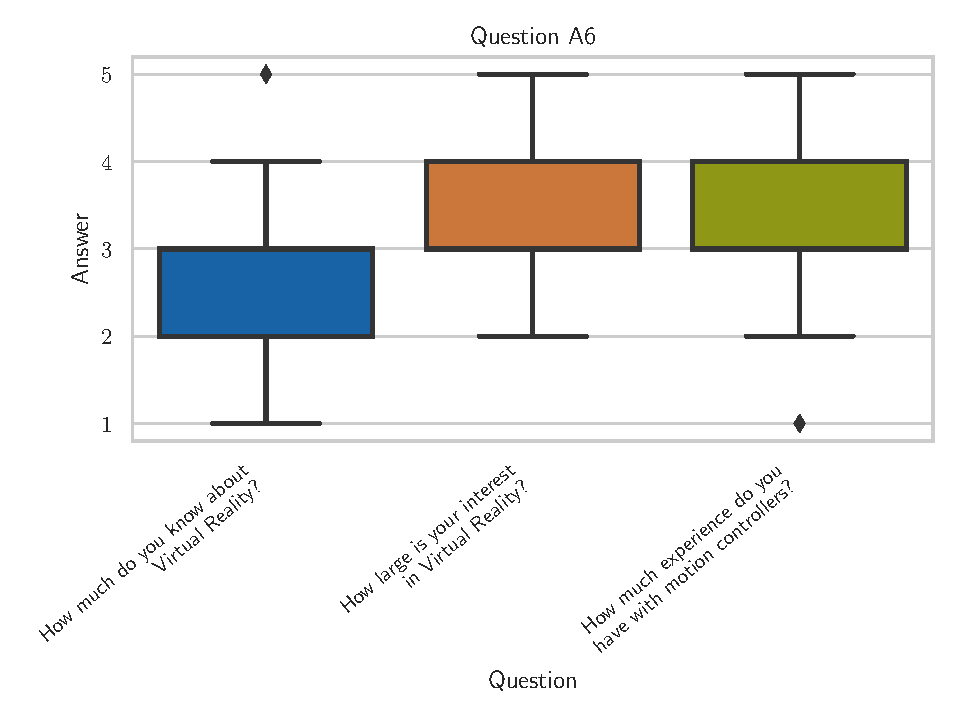
\includegraphics[width=10cm]{figures/evaluation/res_demo_q9.pdf}
	\caption[VR experience of the participants]{Box plots of the answers to the question A6 about the experience of the participants with \gls{VR}. The questions are rated with values ranging from one (\enquote{none}) to five (\enquote{a lot}). While the knowledge about \gls{VR} is rather low (Mean: 2.83; \gls{STD}: 1.03), the interest in the topic \gls{VR} is quite high (Mean: 3.48; \gls{STD}: 0.99). In average participants answered with 3.30 (\gls{STD}: 1.22) as their experience with motion controllers.}\label{fig:res-demo-q9}
\end{figure}

The second question asked about the interest in \gls{VR}, to which no participant answered with \enquote{none} (Mean: 3.48; \gls{STD}: 0.99). The last question asked about the experience with motion controllers. It was explicitly mentioned that the Wii remote counts as a motion controller, which might be the reason for the average, which is higher than the one asking about the knowledge of \gls{VR} (Mean: 3.30; \gls{STD}: 1.22).


\subsection{Model Viewer}\label{section:eval-res-mv}

The model viewer experiment, described in Section~\ref{subsection:model-viewer}, allows users to view a \gls{3D} model from different angles. To benchmark extensive usage, the users had to match the orientation of the model with the orientation of a second model instance in a golden color (the target). After starting the task, the target is spawned with a random orientation.
Since in the current implementation, the model cannot be rotated upside down (as mentioned in Section~\ref{subsection:topic-data}), only reachable target positions are generated.

As soon as the task is started, the user has 30 seconds to match as many orientations as possible. Similar to the implementation by \citeauthor{Katzakis.2010}, the target is rotated to a new random orientation after one orientation was matched~\cite[140]{Katzakis.2010}.
Because it is hard to match the rotation exactly on all three axes, it is enough to pose the model in a similar orientation to the target. A similar pose is reached when the smallest angle between the two rotations is less than 20 radians.

%  T-Test:
%\pgfmathparse{(\evalExpMvAvgPoses-6.5)/(\evalExpMvStdPoses/sqrt(\evalExpMvParticipants))}\pgfmathprintnumber[fixed, precision=2]{\pgfmathresult} 
% chktex 1
\citeauthor{Katzakis.2010} tracked the time it takes to match a pre-defined pose with a smartphone, a mouse, and a touch panel. The lowest time in average to match one pose, 6.5 seconds, was achieved using the smartphone as input device~\cite[140]{Katzakis.2010}. As seen in Figure~\ref{fig:eval-exp-mv}, the average time it took to match a correct pose in the model viewer experiment is roughly \evalExpMvAvgPoses{} seconds, which is lower than the average time of \citeauthor{Katzakis.2010}. This can be due to the fact that users never had to turn the smartphone completely upside down, due to the previously mentioned limitation.

\begin{figure}[H]
	\centering
	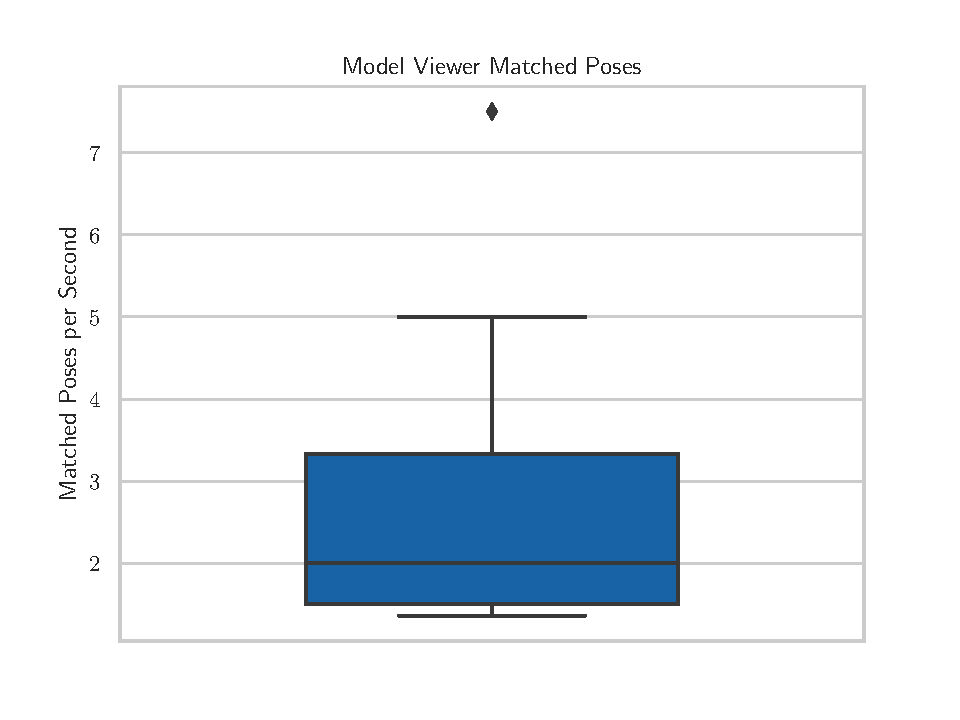
\includegraphics[width=10cm]{figures/evaluation/eval_exp_mv.pdf}
	\caption[Model viewer task results]{A box plot of the time in seconds, it took to match a correct pose in the model viewer experiment.}\label{fig:eval-exp-mv}
\end{figure}

Another reason for the lower average time is that the target and the controlled model are not displayed in two separate locations like in {\citetitle{Katzakis.2010}} by \citeauthor{Katzakis.2010}, but instead with the same origin in the same coordinate space, which makes it easier to see the difference between both rotations~\cite[140]{Katzakis.2010}. Also, the fact that a skeleton model, instead of a multi-colored cube was used, could play a role.

Not only the measured statistics from the experiment but also the \gls{SUS} study results indicate a useable implementation, as seen in Figure~\ref{fig:exp-mv-stats}. A score of \evalExpMvSusScore{} is considered \evalExpMvSusAdj{} and mapped to the grade \evalExpMvSusGrade, according to \citeauthor{Bangor.2009}~\cite[120\psq]{Bangor.2009}.

\begin{figure}[H]
	\centering
	\begin{subfigure}{.48\linewidth}%
		\centering
		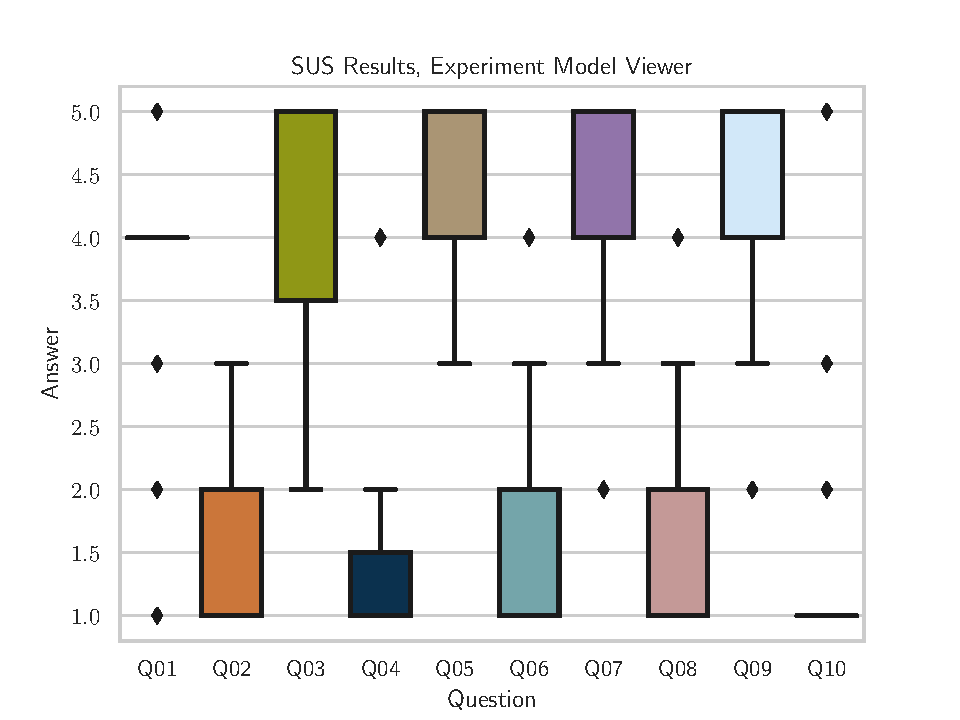
\includegraphics[width=\linewidth]{figures/evaluation/res_exp_mv.pdf}
		\caption{Box plots of the results of question one to ten.}\label{fig:res-exp-mv}
	\end{subfigure}%
	\hspace{0.03\linewidth}%
	\begin{subfigure}{.48\linewidth}%
		\centering
		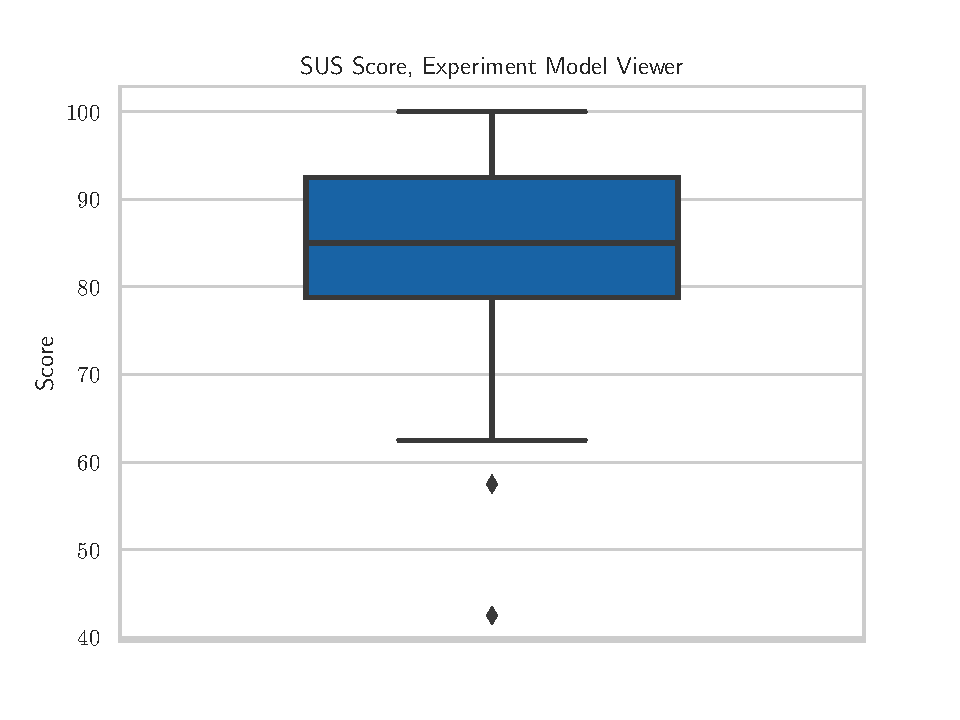
\includegraphics[width=\linewidth]{figures/evaluation/score_exp_mv.pdf}
		\caption{A box plot of the overall \gls{SUS} score.}\label{fig:score-exp-mv}
	\end{subfigure}%
	\caption[Model viewer SUS results]{Box plots of the results of the \gls{SUS} user study for the model viewer.}\label{fig:exp-mv-stats}
\end{figure}

Participants provided additional feedback after the \gls{SUS} user study. They raised the concern that the phone is too large and has a weird shape for controlling a \gls{3D} model on the display. Since every device, similar to a smartphone, with basic web capabilities and sensors, could be used, it would be no problem to use another more comfortable device. 


\subsection{Laser Pointer}\label{section:eval-res-lp}

Section~\ref{subsection:laser-pointer} introduces the laser pointer experiment. To test the performance of participants using this interaction, the participant has to select as many targets as possible in 30 seconds. The user was told to be as fast and especially as accurate as possible since the miss-hits are counted. To trigger a selection, the user has to touch the smartphone display. This counts as a click. If no target was selected, a miss is counted. The total selection (click) count is the sum of hits and miss-clicks.

%Cubes were choosen as target objects, because \gls{UI} elements are often rectangular like the \gls{2D} projection of a cube.
Three cubes (the targets) are spawned at random locations in front of the user. The cubes are always spawned in the view of the user so that the user does not have to look for the targets actively. 
If one cube was hit, another one is spawned, so that always three cubes are visible. This is important because the user can plan to hit the next target while currently aiming for the current one. Otherwise, the task would test the user's reaction time, which is not desired. It was found that three cubes are a good amount, because too much targets would not only clutter the view, but also shorten the aiming periods.

Figure~\ref{fig:eval-exp-lp} visualizes the total click count (Mean: 31.83; \gls{STD}: 6.89), the actual hit count (Mean: 26.13; \gls{STD}: 5.52) and the count of miss-hits (Mean: 5.70; \gls{STD}: 4.37) per 30 seconds. Participants were able to successfully point to and select objects with a speed of nearly one click per second. As seen in Figure~\ref{fig:eval-exp-lp-ratio-scatter}, the hit/miss ratio is very high for slightly lower speeds but decreases fast with higher click speeds.

\begin{figure}[H]
	\centering
	\begin{subfigure}{.48\linewidth}%
		\centering
		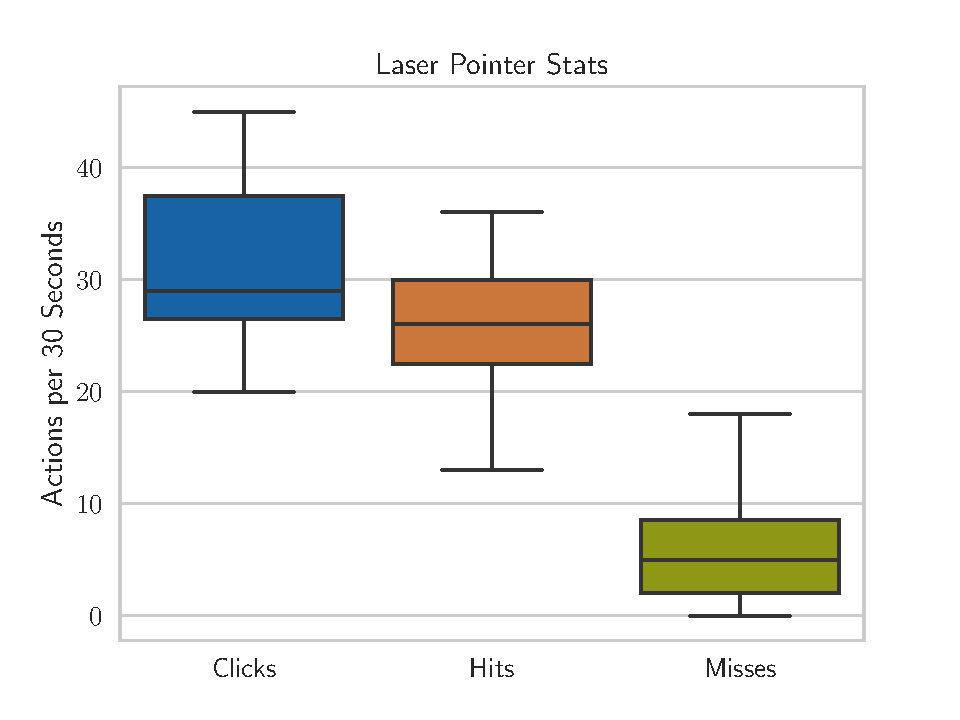
\includegraphics[width=\linewidth]{figures/evaluation/eval_exp_lp.pdf}
		\caption{The count of clicks, hits and misses per 30 seconds. Clicks are the sum of hits and misses.}\label{fig:eval-exp-lp}
	\end{subfigure}%
	\hspace{0.02\linewidth}%
	\begin{subfigure}{.48\linewidth}%
		\centering
		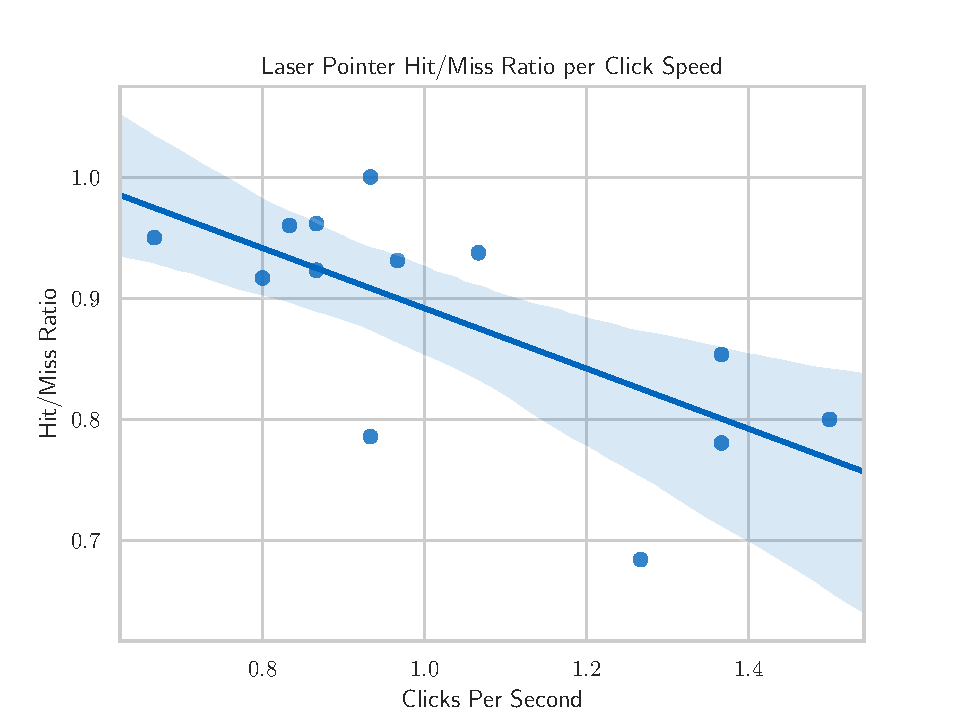
\includegraphics[width=\linewidth]{figures/evaluation/eval_exp_lp_ratio_scatter.pdf}
		\caption{The Hit/Miss ratio per click speed.}\label{fig:eval-exp-lp-ratio-scatter} %The line visualizes the linear regression with a 95\% confidence interval.
	\end{subfigure}%
	\caption[Laser pointer task results]{These figures present the measured statistics of the laser pointer experiment. Participants hit targets more often (Mean: 26.13; \gls{STD}: 5.52) than they missed targets (Mean: 5.70; \gls{STD}: 4.37) in average per 30 seconds. The hit/miss ratio decreases with increasing hit speeds.}\label{fig:exp-lp-eval}
\end{figure}

The performance of this experiment is hard to compare with other implementations without a standardized experiment setup. For example, the size, shape, position, and distance of the targets but also the spawn area and whether distracting elements are present, varies between different task evaluations of other research. However, a comparison should still give a rough estimate of the performance. Often the hit count is measured in different time intervals. To compare the results, the average hit count per second is calculated.

\citeauthor{Kamm.2018} tested his implementation in a similar \gls{VR} scenario with a wrist band as an input device. To compare his implementation, he also tested a laser pointer approach using a \gls{VR} motion controller~\cite[39]{Kamm.2018}. A major difference to his experiment setup is that only one target is displayed at a time. Another difference is that the user has to rotate his head more in order to see the targets as they are placed in a 90 degrees radius. An arrow, which always points to the next target, is displayed to prevent wasting time while searching for the next target. Also, the distance from the user to the targets is randomized~\cite[45]{Kamm.2018}.

\citeauthor{JiYoungOh.2002} compared a real-world laser pointer for large screen interactions to a computer mouse. The application is displayed through a projector, and the laser is detected by a camera. The pointer-device also has a button, which is pressed down to select an object, similar to the laser pointer implementation presented in Chapter~\ref{section:eval-res-lp}. All targets are always visible and have to be selected in a pre-determined order. Also, the fact that all objects are on the same plane makes the task similar to the one presented in this thesis~\cite[3\psq]{JiYoungOh.2002}.

As seen in Table~\ref{tab:lp-comp}, the technique presented in Chapter~\ref{section:eval-res-lp} is the one with the best results. However, due to the different conditions and task setups, it is not possible to draw a strong conclusion. Still, the result is similar to a real-world pointing technique, which is a good sign.

\begin{table}[H]
	\centering
	\begin{tabular}{l c c}
		\toprule
		Source                                            & Average Hits per Second                                                            & Standard Deviation                                                                \\
		\midrule
		\citeauthor{Kamm.2018}~\cite{Kamm.2018}           & \pgfmathparse{\kammAvgHits}\pgfmathprintnumber[fixed, precision=2]{\pgfmathresult} & \pgfmathparse{\kammAvgStd}\pgfmathprintnumber[fixed, precision=2]{\pgfmathresult} \\%chktex 2
		\citeauthor{JiYoungOh.2002}~\cite{JiYoungOh.2002} & $\youngAvgHits{}$                                                                  & $\youngAvgStd{}$                                                                  \\%chktex 2 21
		Chapter~\ref{section:eval-res-lp}                 & \pgfmathparse{\oursAvgHits}\pgfmathprintnumber[fixed, precision=2]{\pgfmathresult} & \pgfmathparse{\oursAvgStd}\pgfmathprintnumber[fixed, precision=2]{\pgfmathresult} \\
		\bottomrule
	\end{tabular}
	\caption[Comparison of laser pointer task results]{This table compares the average hits per second from similar laser pointer evaluations of other research. The implementation from Chapter~\ref{section:eval-res-lp} achieved the highest average hits per second.}\label{tab:lp-comp}
\end{table}

Not only the measured interaction times but also the \gls{SUS} study results indicate a useable implementation, as seen in Figure~\ref{fig:exp-lp-stats}. A score of \evalExpLpSusScore{} is considered \evalExpLpSusAdj{} and mapped to the grade \evalExpLpSusGrade{}, according to \citeauthor{Bangor.2009}~\cite[120\psq]{Bangor.2009}.

\begin{figure}[H]
	\centering
	\begin{subfigure}{.48\linewidth}%
		\centering
		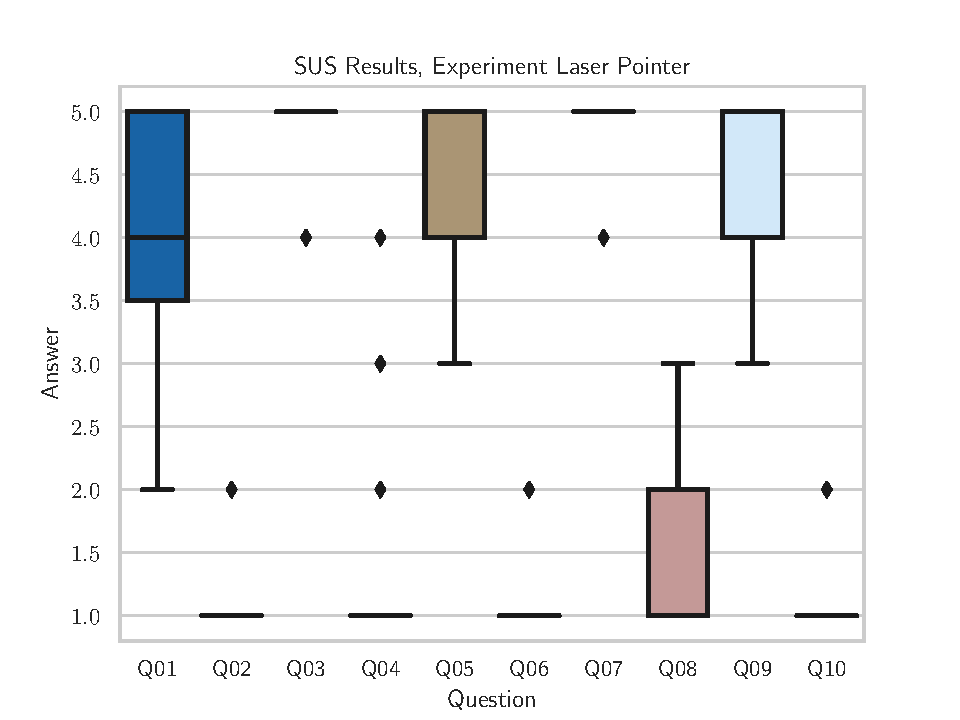
\includegraphics[width=\linewidth]{figures/evaluation/res_exp_lp.pdf}
    \caption{The results of question one to ten presented as box plots.}\label{fig:res-exp-lp}
	\end{subfigure}%
	\hspace{0.04\linewidth}%
	\begin{subfigure}{.48\linewidth}%
		\centering
		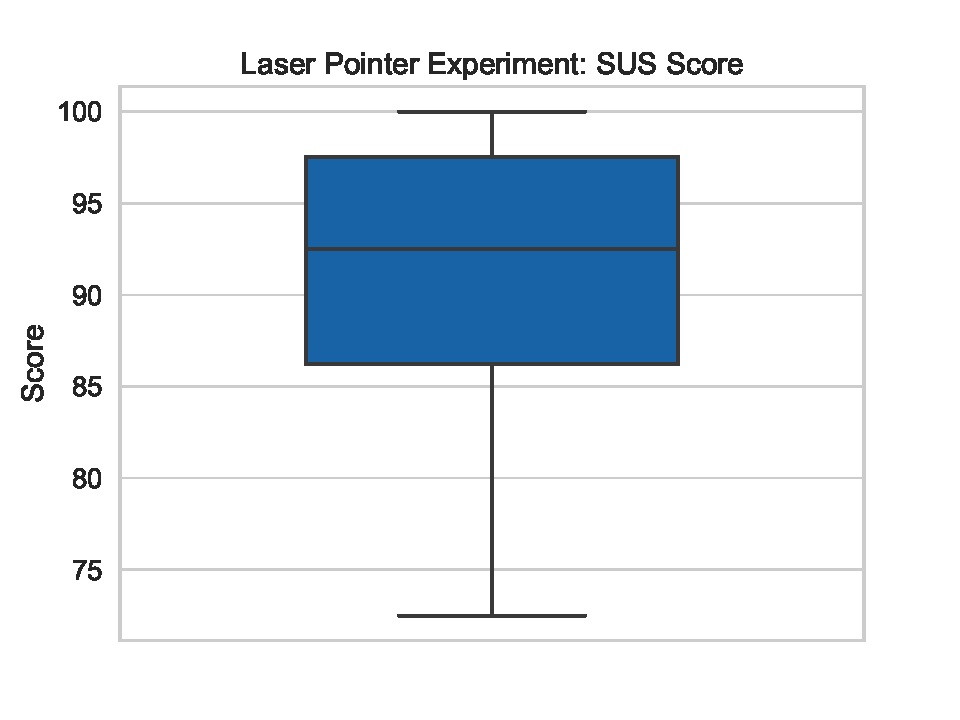
\includegraphics[width=\linewidth]{figures/evaluation/score_exp_lp.pdf}
		\caption{The overall \gls{SUS} score presented in a box plot.}\label{fig:score-exp-lp}
	\end{subfigure}%
	\caption[Laser pointer SUS results]{The results of the \gls{SUS} user study for the laser pointer. Ignoring a few outliers, participants agree on most \gls{SUS} questions clearly, as seen in Figure~\ref{fig:res-exp-lp}.}\label{fig:exp-lp-stats}
\end{figure}

Some participants mentioned that it is hard to notice whether the laser pointer is going to hit an object or not. They suggested better indicators, like a bigger laser beam or an indicator at the position, where the laser hits an object.


\subsection{Virtual Keyboard}\label{section:eval-res-vk}

The task for the virtual keyboard experiment, presented in Chapter~\ref{subsection:virtual-keyboard}, is to enter a text as fast as possible without mistakes. The text chosen for this task is \enquote{A quick brown fox jumps over the lazy dog}, which is commonly used when testing keyboards, typewriters or fonts because it contains all characters of the alphabet.

To test the \enquote{shift}-key more than just with the first capitalized letter, also an exclamation mark is added at the end. This given text is displayed on top of the text which is currently typed with the keyboard. If a mistake was made, it has to be corrected in order to complete the task. After starting the task, a timer counts the time until the \enquote{enter}-button is pressed.

The count of corrections the participants made while entering the given text has an average of 2.7 (mean: 2.74; \gls{STD}: 2.38). A correction is counted when the user uses the \enquote{backspace}-key to remove one character. If he did not recognize his error soon enough, it is possible that in order to correct one letter, the user has to remove multiple characters which are counted as multiple \enquote{corrections}. Since the participant has to type a total of 42 characters, the average correction count to character count ratio is at 6.52\%.
Participants took 31.7 seconds on average (\gls{STD}: 5.1) to complete the task. Figure~\ref{fig:eval-exp-vk-ratio-scatter} shows that the more mistakes were made, the more time users needed to complete the task.

\begin{figure}[H]
	\centering
	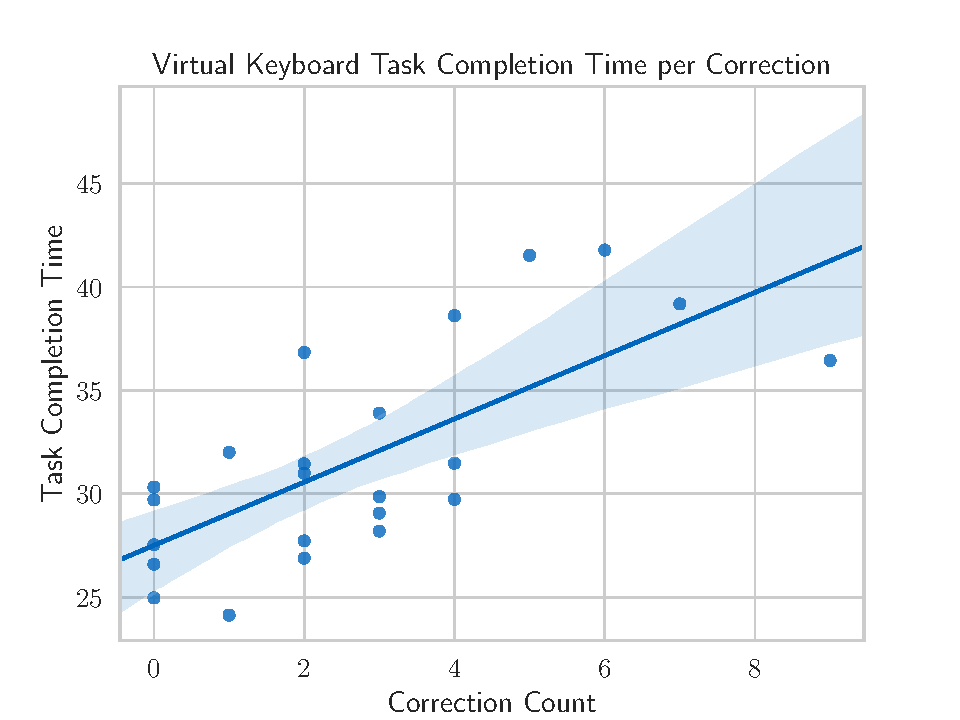
\includegraphics[width=10cm]{figures/evaluation/eval_exp_vk_ratio_scatter.pdf}
	\caption[Virtual keyboard task results]{A scatter plot of the time it took to complete the virtual keyboard task per correction count. The line visualizes the linear regression with a 95\% confidence interval. The more corrections were made, the longer participants took to complete the task.}\label{fig:eval-exp-vk-ratio-scatter}
\end{figure}

The \gls{SUS} score for this experiment, shown in Figure~\ref{fig:exp-mv-stats}, is \evalExpVkSusScore{}.
According to \citeauthor{Bangor.2009}, this score is considered \evalExpVkSusAdj{} and mapped to the grade \evalExpVkSusGrade~\cite[120\psq]{Bangor.2009}. Since this score is still in the \enquote{acceptable} range~\cite[120\psq]{Bangor.2009}, it can be considered \enquote{usable}.

\begin{figure}[H]
	\centering
	\begin{subfigure}{.5\linewidth}%
		\centering
		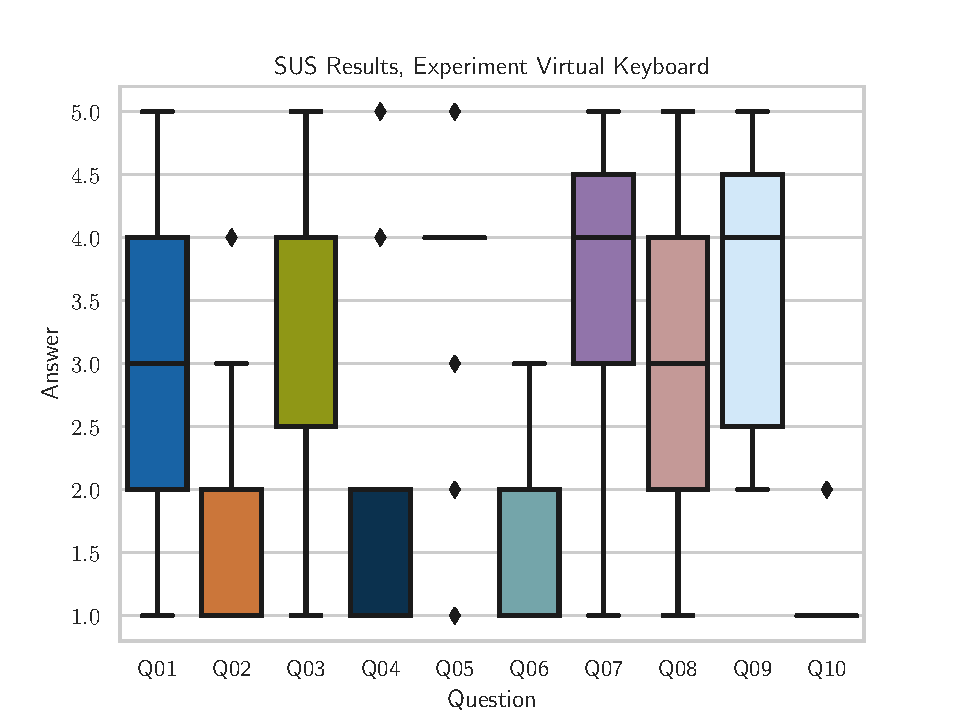
\includegraphics[width=\linewidth]{figures/evaluation/res_exp_vk.pdf}
		\caption{Box plots of the results of question one to ten.}\label{fig:res-exp-vk}
	\end{subfigure}%
	\begin{subfigure}{.5\linewidth}%
		\centering
		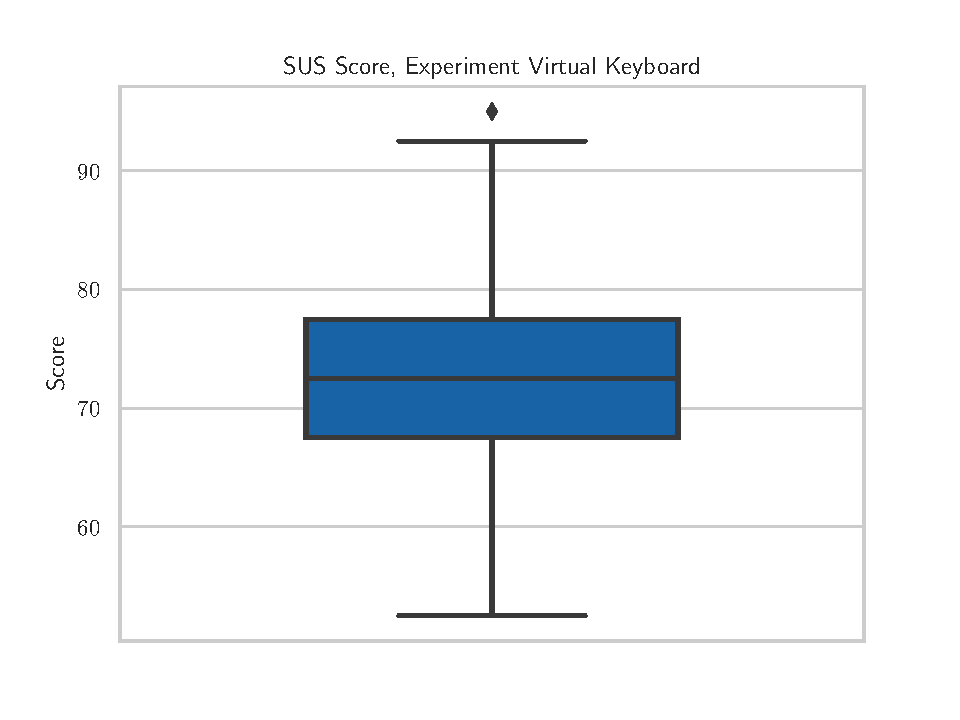
\includegraphics[width=\linewidth]{figures/evaluation/score_exp_vk.pdf}
		\caption{A box plot of the overall \gls{SUS} score.}\label{fig:score-exp-vk}
	\end{subfigure}%
	\caption[Virtual keyboard SUS results]{Box plots of the results of the \gls{SUS} user study for the virtual keyboard.}\label{fig:exp-vk-stats}
\end{figure}

Further, many users made comments about the experiment:
\begin{itemize}
	\item The sensitivity of the movement detection should be decreased.
	\item A faster selection speed would improve comfort and typing speed.
	\item Visual, audible or vibrational feedback after typing a character would be great.
	\item The one to one mapping of the display to the virtual keyboard is not very intuitive.
	\item A cursor in the input text should be displayed, to visualize spaces. Also, arrow keys to navigate through the text would be handy.
	\item To improve usability, select buttons when the finger releases the touch screen, instead of waiting.
	\item It should be possible to use multiple fingers at the same time.
	\item An implementation like the Swift-keyboard for Android might be a better one, since holding the finger down was cumbersome.
	\item Another approach would be to paint characters on the screen using the touch screen, or the laser pointer.
\end{itemize}

% !TeX root = ../main.tex
% important chapter: spell out acronyms like in abstract
\chapter{Conclusion}\label{chapter:conclusion}

To show that the smartphone is a valuable device for interacting with \glsentrylong{VR}, typical input methods used in \glsentrylong{VR} were explored and evaluated. A \glsentrylong{SUS} study showed that all three experiments, the model viewer, the laser pointer and the virtual keyboard experiment, were usable. %TODO: grammarly

Three-dimensional models can be viewed with the model viewer experiment. In the evaluation most participants agreed that this input method is intuitive to operate.

The laser pointer is used to select elements in a \glsentrylong{UI} or for similar pointing tasks. This experiment scored the highest amongst the ones presented in this thesis. 

The virtual keyboard experiment, solves the problem of typing text while being immersed in a \glsentrylong{VE}. While the model viewer and the laser pointer scenario reached a high score, the virtual keyboard scored slightly lower. 

A lot of feedback was collected during the survey, which can be used to improve these implementations further. Since all implementations are considered \enquote{acceptable}, it can be assumed that the smartphone is indeed a helpful input device for \glsentrylong{VR}.

The implementation used the \glsentrylong{UBII} system to abstract parts of the application, which makes the system more modular and extensible. This was achieved by implementing logic into \enquote{Interactions}, which are processed on the server. 

% !TeX root = ../main.tex
\phantomsection{}
\addcontentsline{toc}{chapter}{Acknowledgments}
\thispagestyle{empty}

\vspace*{20mm}

\begin{center}
{\usekomafont{sectioning}\usekomafont{section} Acknowledgments}
\end{center}

\vspace{10mm}

Foremost, I would like to thank my supervisor \getSupervisor\ at \getUniversity\ for giving me the opportunity to write my bachelor's thesis at her chair Forschungsgruppe Augmented Reality.

I would also like to express my sincere gratitude to my advisor, \getAdvisor\ for the close supervision and helpful advice.

A special thank goes to all my friends who took the time to participate in the evaluation.

Last but not least, I would like to thank my family for their continuous support during my studies and the writing of this thesis.

\cleardoublepage{}


\microtypesetup{protrusion=false}
\listoffigures{}
\listoftables{}
\microtypesetup{protrusion=true}

% !TeX root = ../main.tex

\begin{appendices}
  % Evaluation Devices
  \chapter{User Evaluation Devices}\label{chapter:append-user-eval-devices}
  \section{Testing Environment A: Home}
  \begin{itemize}
    \item Smartphone
    \begin{itemize}
      \item Type: ONEPLUS A6013
      \item \gls{OS}: Android 9
      \item RAM: 8 GB
      \item CPU: Snapdragon 845 % chktex 36
      \item Web browser: Firefox Android, Version 68.0
    \end{itemize}
    \item \gls{PC}
    \begin{itemize}
      \item \gls{OS}: Windows 10
      \item RAM: 32 GB
      \item CPU: Intel Core i7-6700K % chktex 36 chktex 8
      \item GPU: NVIDIA GeForce GTX 1080
      \item Storage: Intel SSD 535 Series, 480GB
      \item Web browser: Firefox Standard Release, Version 68.0.1
    \end{itemize}
    \item \gls{HMD}
    \begin{itemize}
      \item Oculus Rift, Consumer Version 1
    \end{itemize}
  \end{itemize}

  \filbreak{}
  \section{Testing Environment B: University}
  \begin{itemize}
    \item Smartphone
    \begin{itemize}
      \item Type: ONEPLUS A6013
      \item \gls{OS}: Android 9
      \item RAM: 8 GB
      \item CPU: Snapdragon 845 % chktex 36
      \item Web browser: Firefox Android, Version 68.0
    \end{itemize}
    \item \gls{PC}
    \begin{itemize}
      \item \gls{OS}: Windows 10 Enterprise
      \item RAM: 32 GB
      \item CPU: Intel Core i5-8600K % chktex 36 chktex 8
      \item GPU: NVIDIA GeForce GTX 1080 Ti
      \item Storage: Samsung SSD 860 EVO, 500GB
      \item Web browser: Firefox Standard Release, Version 68.0.1
    \end{itemize}
    \item \gls{HMD}
    \begin{itemize}
      \item HTC Vive Pro with SteamVR 2.0 Lighthouse
    \end{itemize}
  \end{itemize}

  % Assets
  \chapter{External Assets Used}\label{chapter:external-assets-used}
  
  For demonstration purposes, assets from external sources where used. The licenses were reviewed to determine whether the use and modification in the context of this research is legally possible. All resources were modified by the author of this thesis.

  Icons used in the diagrams:
  \begin{itemize}
    \item Icons from \href{https://www.draw.io/}{draw.io} by JGraph Ltd.\\Terms: \href{https://desk.draw.io/support/solutions/articles/16000039574-draw-io-eula-terms-of-service}{desk.draw.io/support/solutions/articles/16000039574-draw-io-eula-terms-of-service}
  \end{itemize}

  Three-dimensional models used in the experiments:
  \begin{itemize}
    \item Simple Rigged Skeleton by Gord Goodwin (CC0).\\Source: \href{http://gord-goodwin.blogspot.com/2010/03/manny-mannequin.html}{www.gord-goodwin.blogspot.com/2010/03/manny-mannequin.html}
    \item Smartphone by Brian MacIntosh (CC0).\\Source: \href{https://opengameart.org/content/smartphone-1}{www.opengameart.org/content/smartphone-1}
  \end{itemize}


  % Evaluation Form
  \includepdf[pages=1,pagecommand={\chapter{User Evaluation Form}\label{chapter:append-user-eval-form}},width=\textwidth,clip,trim=0mm 9cm 0mm 0mm]{appendices/evaluation.pdf} % the trimming is not supported with XeLaTeX
  \includepdf[pages=2-,pagecommand={},width=\textwidth]{appendices/evaluation.pdf}
\end{appendices}
\printbibliography{}



\end{document}
